\documentclass[usenames,dvipsnames,french]{beamer}

\mode<presentation> {

\usetheme{Montpellier}
}

\usepackage{graphicx} % Allows including images
\usepackage[frenchb]{babel}
\usepackage[T1]{fontenc}
\usepackage[utf8]{inputenc}
% \usepackage[demo]{graphicx}
% \usepackage{caption}

\usepackage{subcaption}
% \usepackage{subfig}
% \usepackage{algorithm,algorithmic}
\usepackage{algorithm2e}
\usepackage{listings}
% \usepackage{ntheorem}
\usepackage{booktabs} % Allows the use of \toprule, \midrule and \bottomrule in tables
\setcounter{tocdepth}{2}
\graphicspath{{../../Figures/}}


% exercices comptés
\newcounter{numexos}%Création d'un compteur qui s'appelle numexos
\setcounter{numexos}{0}%initialisation du compteur
\newcommand{\exercice}[1]{%Création d'une macro ayant un paramètre
\addtocounter{numexos}{1}%chaque fois que cette macro est appelée, elle ajoute 1 au compteur numexos
\textcolor{DarkOrchid}{Exercice\,\thenumexos\,:}\,#1%Met en rouge Exercice et la valeur du compteur appelée par \thenumeexos
}
%----------------------------------------------------------------------------------------
%	TITLE PAGE
%----------------------------------------------------------------------------------------

\setbeamertemplate{title page}{
    \centering

    \Large\bfseries
    Machine learning Tek 5: reinforcement learning
    

\begin{figure}[!h]
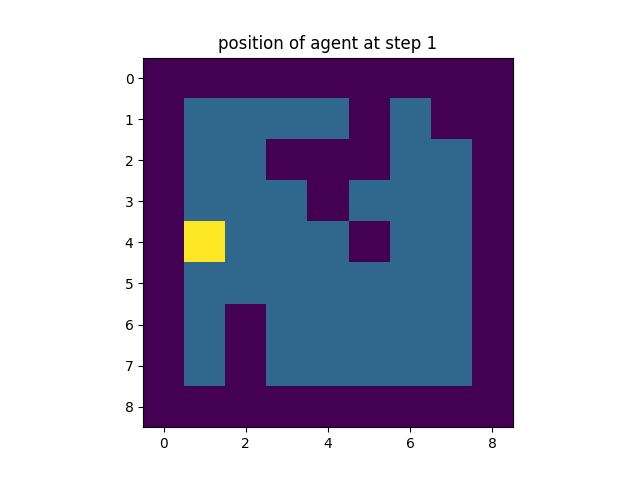
\includegraphics[width=8cm]{agent_position_travel_3_step_1}
\end{figure}

    }
\begin{document}

\frame{\titlepage}

\section{Presentation of Reinforcement Learning}%
\label{sec:section_name}



\begin{frame}
    \begin{itemize}
        \item RL has many applications and \textbf{{Deep Reinforcement Learning}} has received a lot of attention for more than 10 years now.

	    \item Sutton textbook: \url{http://incompleteideas.net/book/the-book-2nd.html} 
    \end{itemize}
\end{frame}

\begin{frame}
    \begin{itemize}
        \item Atari games
	    \begin{figure}[htpb]
	        \centering
	        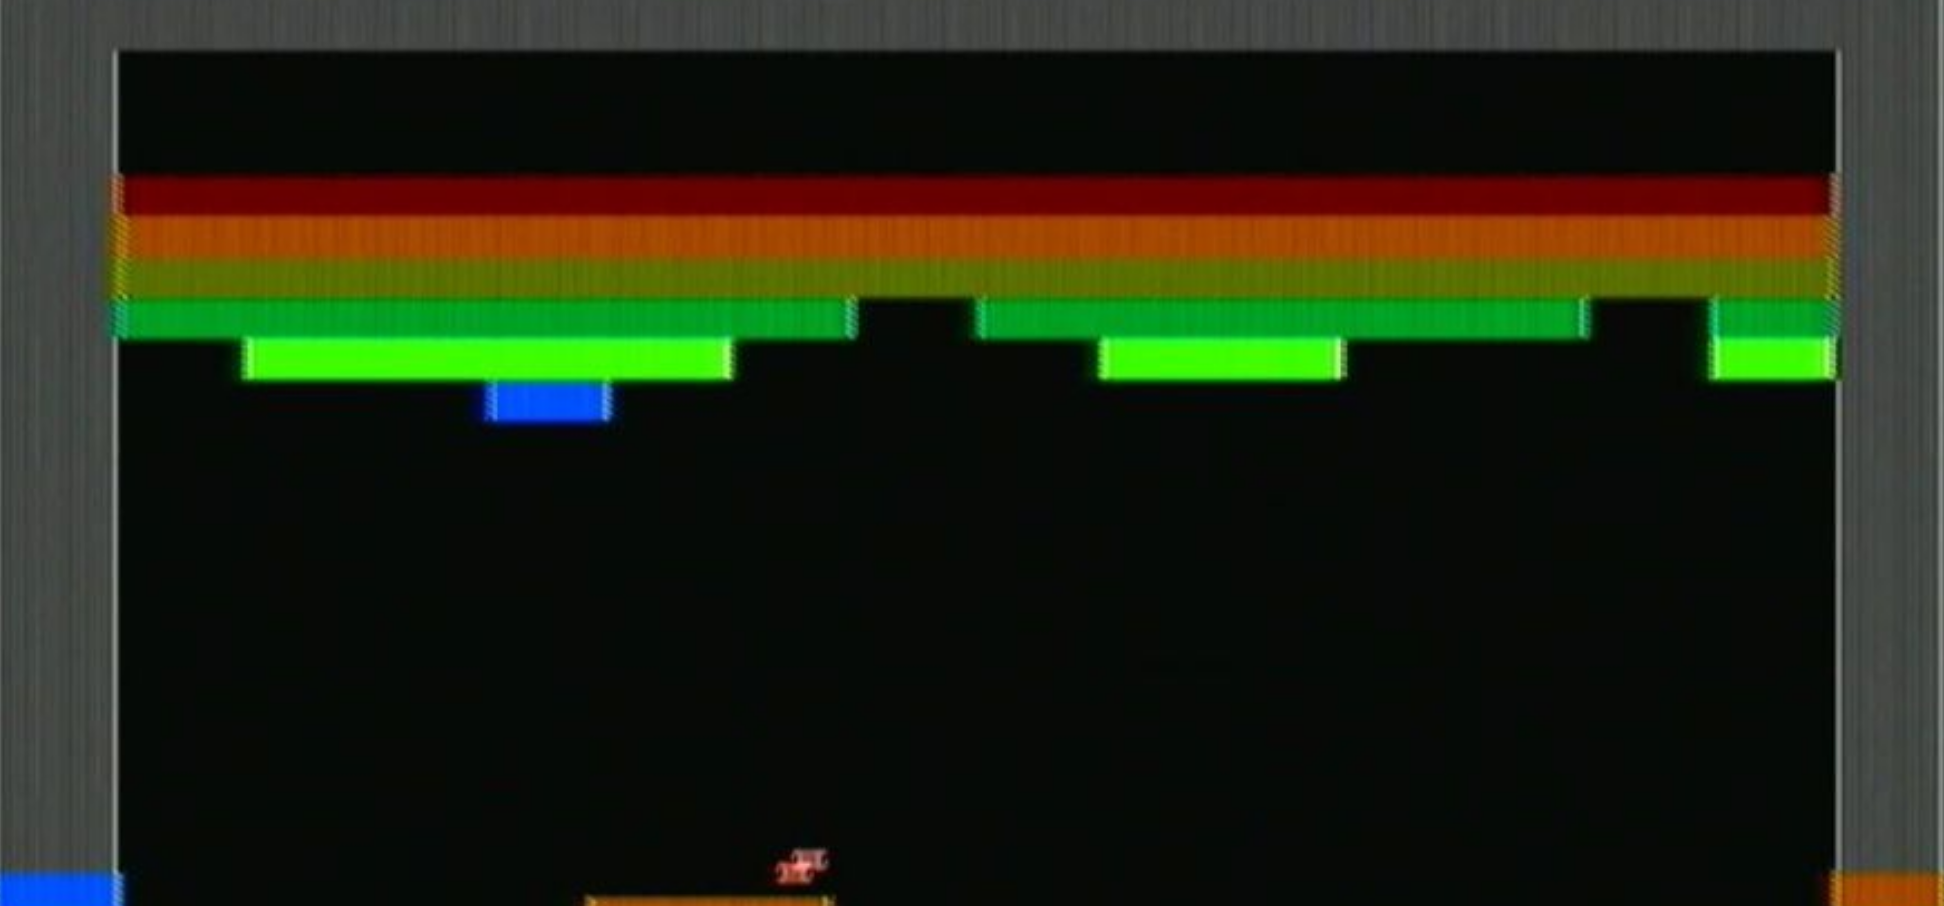
\includegraphics[width=0.8\linewidth]{atari}
		\caption{\cite{Mnih2013}}
	        \label{fig:}
	    \end{figure}
    \end{itemize}
\end{frame}


\begin{frame}
    \begin{itemize}
        \item AlphaGo
	    \begin{figure}[htpb]
	        \centering
	        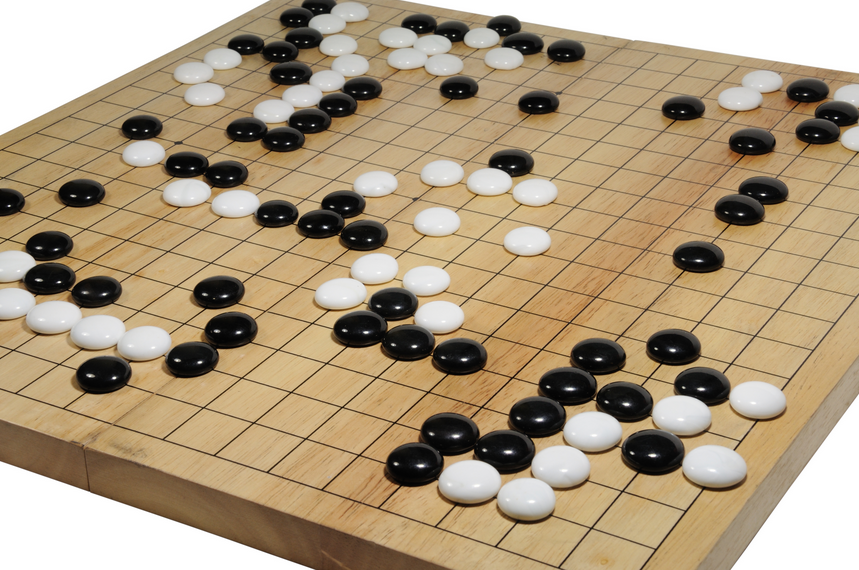
\includegraphics[width=0.8\linewidth]{go}
	        \caption{Go game, beaten by AlphaGo in 2017 \cite{SilverHuangEtAl16nature}}
	        \label{fig:go}
	    \end{figure}
    \end{itemize}
\end{frame}

\begin{frame}
    \begin{itemize}
        \item Reinforcement Learning is also being used in the community of \textbf{{Computationnal neuroscience.}} 
    \end{itemize}
\end{frame}

\section{The framework}%
\label{sec:j}

\subsection{Supervised learning}%
\label{sub:supervised_learning}


\begin{frame}{Supervised learning and Correction}
    \begin{itemize}
        \item In \textbf{{supervised learning}}, the supervisor indicates the \textbf{{expected answer}} the model should answer.
	\item The feedback does not depend on the action performed by the model (for instance the prediction from the model)
	\item We say that the model receives an \textbf{{instructive feedback}}.
	\item The model must then \textbf{{update itself}}  based on this answer.
    \end{itemize}
\end{frame}

\subsection{Reinforcement learning}%
\label{sub:reinforcement_learning}

\begin{frame}{Cost sensitive learning}
   \begin{itemize}
       \item In \textbf{{Cost sensitive learning}}, the situation is different. 
	\item The agent receives an \textbf{{evaluative feedback}}. The feedack depends on the action performed by the agent.
	\item \textbf{{Examples : }}
	    \begin{itemize}
	    \item AI playing a game and receiving "victory" or "defeat" as a feedback.
	    \item Child playing with a toys.
	\end{itemize} 
   \end{itemize} 
\end{frame}

\begin{frame}{Reinforcement learning}
   \begin{itemize}
       \item \textbf{{Reinforcement learning}} is a particular case of cost-sensitive learning.
	\item In reinforcement learning, the feedback is a \textbf{{real number}}.
	\item \textbf{{Example : }} amount of coins won after a poker turn.
   \end{itemize} 
\end{frame}

\begin{frame}{Reinforcement learning}
   \begin{itemize}
	\item First, the agent does not know if a reward is good or bad \textit{per se}.
	\item A reward of $-10$ can be good or bad depending on the other rewards
        that are possible to obtain !
   \end{itemize} 
\end{frame}

\begin{frame}{Reinforcement learning}
   \begin{itemize}
	\item First, the agent does not know if a reward is good or bad per se.
	\item A reward of $-10$ good be good or bad depending on the other rewards that are possible to obtain.
	\item Most of the time, the objective of the agent will be to optimize the \textbf{{agregation of rewards}}.
   \end{itemize} 
\end{frame}

\begin{frame}{Reinforcement learning}
   \begin{itemize}
       \item The agent lives in a world $E$, and can be in several states $s$. The agent performs \textbf{{actions}} $a$ and receives rewards $r$.
	   \item \textbf{{Examples : }} \begin{itemize}
		   \item world = $ \mathbb{R}^2$ 
	       \item state $=$ position
		\item actions $=$ moving somewhere
		\item reward $=$ amount of food found
	   \end{itemize}
   \end{itemize} 
\end{frame}

\begin{frame}{Formalization}
   \begin{itemize}
       \item There are many aspects of the problem that we need to formalize. Several formalizations are possible depending on the situation.
	\item We will consider \textbf{{discrete spaces}} : 
	    \begin{itemize}
	        \item the time will be discrete
		\item the number of possible states will be \textbf{{finite}} 
		\item the number of possible actions will be \textbf{{finite}} 
	    \end{itemize}
    \item Continuous spaces are also available for RL. In those cases the
        objects are slightly different, and the optimization procedures also
           differ. For an introductory course, discrete spaces are more
           suitable.
   \end{itemize} 
\end{frame}

\begin{frame}{Question}
    \begin{itemize}
	\item We will consider \textbf{{discrete spaces}} : 
	    \begin{itemize}
	        \item the time will be discrete
		\item the number of possible states will be \textbf{{finite}} 
		\item the number of possible actions will be \textbf{{finite}} 
	    \end{itemize}
        \item Are these hypotheses valid in the case of AlphaGo ?
	    \begin{figure}[htpb]
	        \centering
	        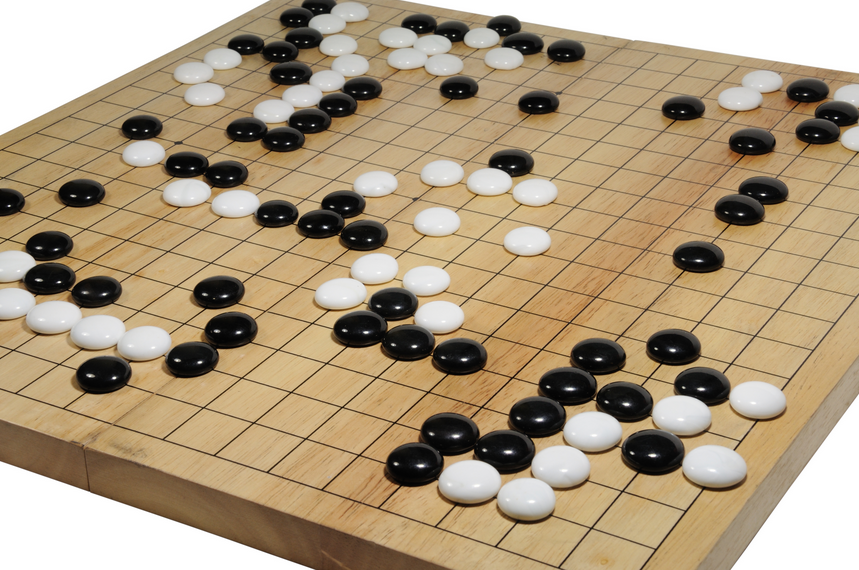
\includegraphics[width=0.4\linewidth]{go}
	        \label{fig:go}
	    \end{figure}
    \end{itemize}
\end{frame}

\begin{frame}{Question}
    \begin{itemize}
	\item We will consider \textbf{{discrete spaces}} : 
	    \begin{itemize}
	        \item the time will be discrete
		\item the number of possible states will be \textbf{{finite}} 
		\item the number of possible actions will be \textbf{{finite}} 
	    \end{itemize}
        \item Are these hypothesis valid in the case of AlphaGo ?
	    \begin{figure}[htpb]
	        \centering
	        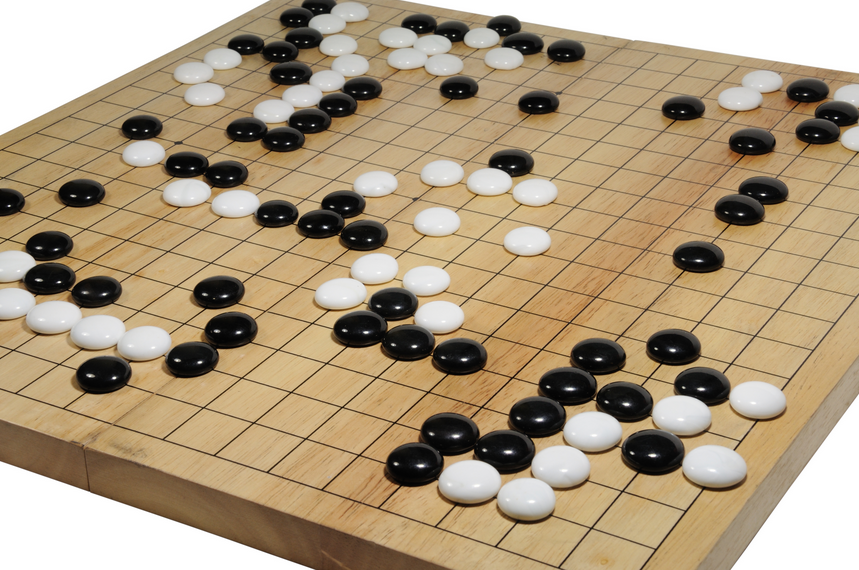
\includegraphics[width=0.3\linewidth]{go}
	        \label{fig:go}
	    \end{figure}
	    \item Yes ! This shows that discrete spaces can still describe very
            complex problems.
    \end{itemize}
\end{frame}

\begin{frame}{Formalization}
   \begin{itemize}
       \item we will write : 
	   \begin{itemize}
	       \item $S_t$ : state at time $t$
	       \item $R_t$ : reward received at time $t$
	       \item $A_t$ : action performed at time $t$
	   \end{itemize}
	\item the actions are chosen according to a \textbf{{policy}} $\pi$
   \end{itemize} 
\end{frame}

\begin{frame}[t]
    \frametitle{Action - reward loop}

    \begin{figure}[htpb]
        \centering
        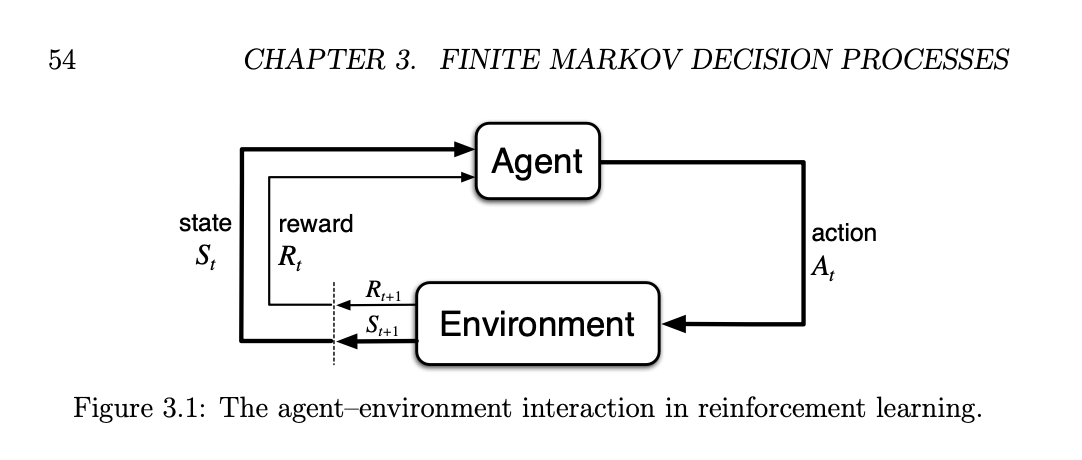
\includegraphics[width=0.8\textwidth]{rlbook}
        \caption{Image taken from the Sutton book, page 68.}
        \label{fig:}
    \end{figure}

    \url{http://incompleteideas.net/book/the-book-2nd.html}
    
\end{frame}

\begin{frame}{Policies}
        The policy is a map that determines the action chosen by the agent. $\pi$ is a function of the current state.
   \begin{itemize}
	\item It can be \textbf{{deterministic :}} the action chosen is chosen with
        probability $1$.
	\item Or \textbf{{stochastic :}} the action performed in a given state is
        drawn from a \textbf{{distribution}}.
   \end{itemize} 
\end{frame}

\begin{frame}{Two levels of randomness}
   \begin{itemize}
	   \item The policy can be deterministic or stochastic.
	    \item But the result of an action could also be stochastic ! This is called a \textbf{{stochastic transition function}}.
   \end{itemize} 
\end{frame}


\begin{frame}{Two levels of randomness}
   \begin{itemize}
	   \item The policy can be deterministic or stochastic.
	    \item But the result of an action could also be stochastic ! This is called a \textbf{{stochastic transition function}}.
		\begin{figure}[htpb]
		    \centering
		    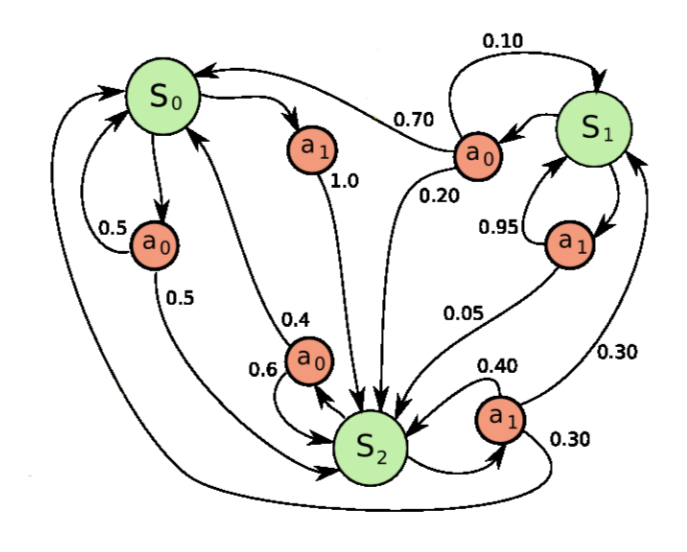
\includegraphics[width=0.6\linewidth]{stopo}
		    \caption{A stochastic policy with a stochastic transition function.}
		    \label{fig:stopo}
		\end{figure}
   \end{itemize} 
\end{frame}

\begin{frame}
    \exercice{}
   \begin{itemize}
       \item What is the probability of staying in state $S_0$ when performing an action from $S_0$ ? and from $S_1$ and $S_2$ ?
	   \begin{figure}[htpb]
	       \centering
	       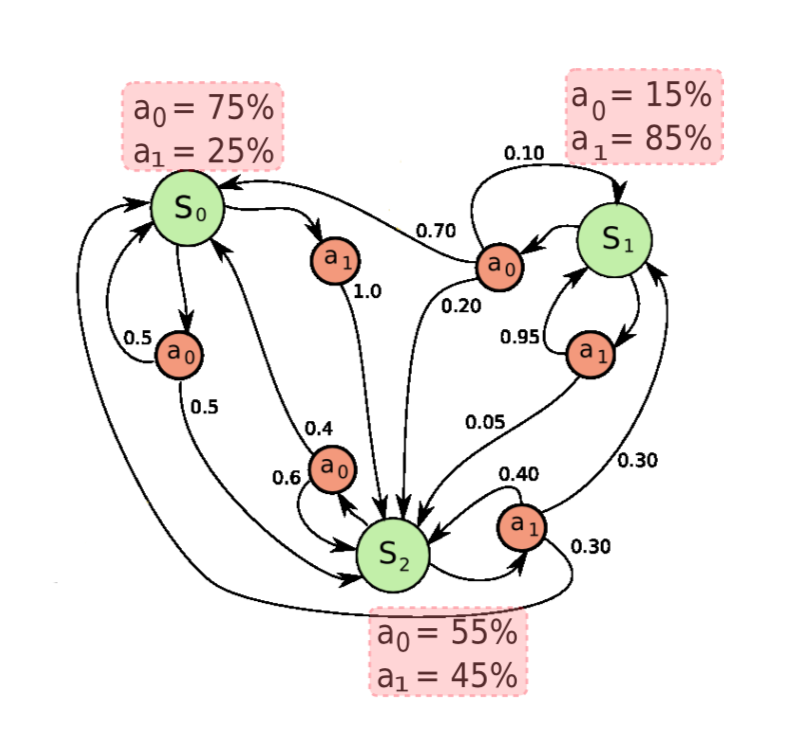
\includegraphics[width=0.5\linewidth]{stopo2}
	       \caption{A stochastic policy with a stochastic transition function.}
	       \label{fig:stopo}
	   \end{figure}
   \end{itemize} 
\end{frame}

\begin{frame}{Agregation of rewards}
   \begin{itemize}
       \item The agent wants to optimize the \textbf{{agregation of the rewards.}} 
	\item There are several ways to agregate the rewards.
   \end{itemize} 
\end{frame}

\begin{frame}{Returns}

    We introduce the \textbf{return} $G_t$.

    \begin{itemize}
	\item Episodic case (finite number $N$ of steps):
	    \begin{equation}
		G_t = R_{t+1} + R_{t+2} + \dots + R_{t+N}
	    \end{equation}
	\item Continuing tasks:
	    \begin{equation}
		G_t = R_{t+1} + \gamma R_{t+2} + \gamma^2 R_{t+3} + \dots 
	    \end{equation}
	    $\gamma \in [0,1[$ is the \textbf{{discount factor}}
    \end{itemize}

\end{frame}

\begin{frame}{Value function}

    Given a fixed policy $\pi$, the value function $v_{\pi}(s)$ quantifies how good a state $s$ is.

    \begin{equation}
	v_{\pi}(s) = E[G_t|S_t=s]
    \end{equation}

    (the expectation is taken over the next actions, following the policy $\pi$).
    \begin{itemize}
        \item $G_t$: return obtained after the word is in state $s$ at time $t$.
	\item $E$: expected value
    \end{itemize}

    \textbf{The value function is unknown first, this is what we want to learn !}

\end{frame}

\begin{frame}{The Bellman equation}

    Given a fixed policy $\pi$, and a state $s$, we can write a recursive relationship between 
    $v_{\pi}(s)$ and the values $v_{\pi}$ of the next possible successor states (see the Sutton book for the general form 
    of the equation 3.12 page 85).

\end{frame}

\begin{frame}{Markov hypothesis}
    A assumption necessary to enable computations, but not always exactly true.

    \url{https://en.wikipedia.org/wiki/Markov_property} 
\end{frame}


\begin{frame}{$\epsilon$-greedy policy}

    A way to tackle the \textbf{exploitation-exploration compromise}.

    \begin{itemize}
        \item with probability $1-\epsilon$: go to the best known reward (exploitation).
        \item with probability $\epsilon$: perform a random action (exploration).
    \end{itemize}

    "RL is a science, but dealing with the exploration-exploitation compromise is an art" (Sutton)

\end{frame}

\section{Dynamic programming}%
\label{sec:dynamic_programming}

\begin{frame}{Dynamic programming}
    \begin{itemize}
        \item Today we will study a simple case of Reinforcement learning
	\item Deterministic transition function.
    \end{itemize}
\end{frame}

\begin{frame}{World}
   \begin{figure}[htpb]
       \centering
       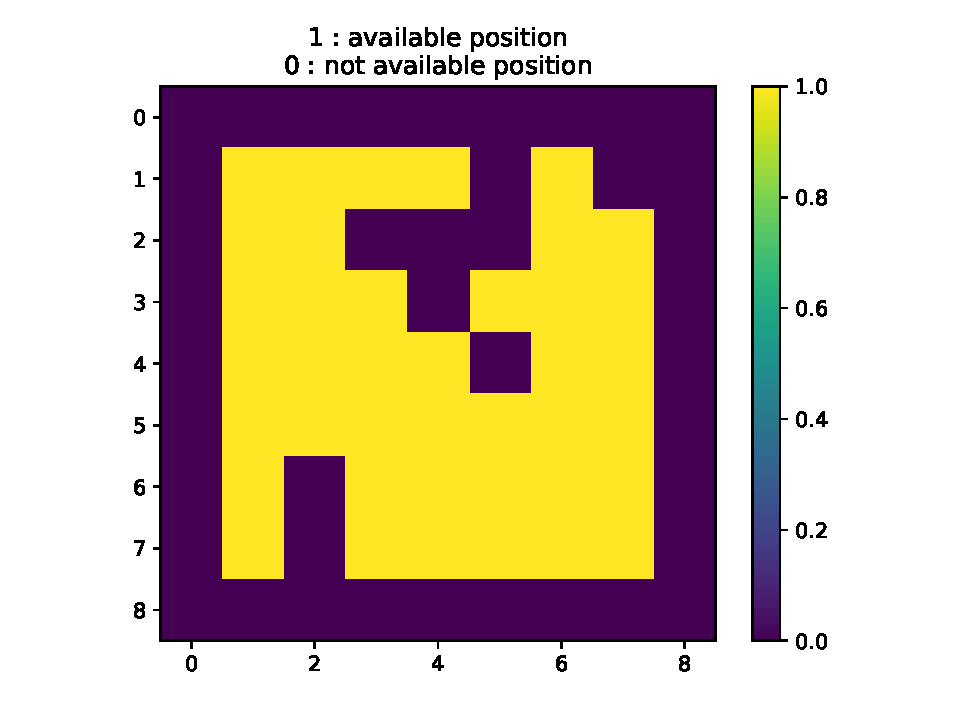
\includegraphics[width=0.6\linewidth]{world}
       \caption{2 dimensional world.}
       \label{fig:world}
   \end{figure}
\end{frame}

\begin{frame}{Reward}
   \begin{figure}[htpb]
       \centering
       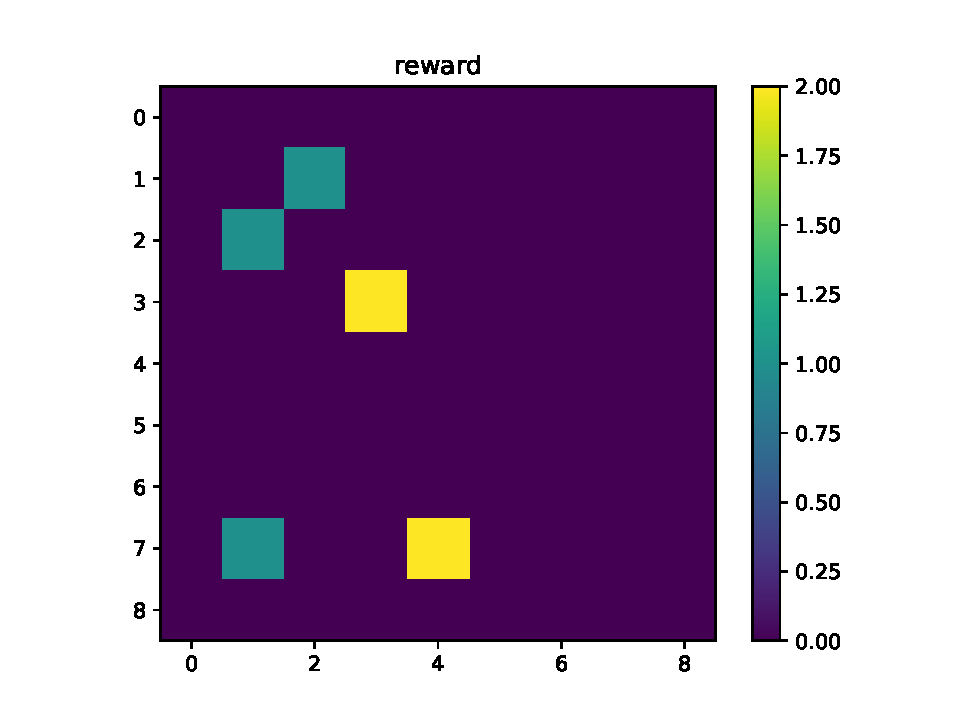
\includegraphics[width=0.6\linewidth]{reward}
       \caption{Reward function.}
       \label{fig:reward}
   \end{figure}
\end{frame}

\begin{frame}{2D world}
\begin{itemize}
    \item Our agent can move to the $8$ neighbor positions (if the positions are available)
\end{itemize}	
\end{frame}

\begin{frame}{Optimal value functions}

    We look for the value of the \textbf{optimal policy} $\pi^*$, defined by the fact that
    it has the best value function among all policies.

\end{frame}

\begin{frame}{Bellmann optimality equation}

           \begin{equation}
	       \begin{aligned}
	       	\label{eq:bellman_opt}
		   v_*(s) &= \max_{a\in\text{available actions}} E[G_t|S_t=s, A_t=a]\\
			    &= \max_{a\in\text{available actions}} E[\sum_{k\geq 0}\gamma^kR_{t+k+1}|S_t=s, A_t=a]\\
			    &= \max_{a\in\text{available actions}} E[R_{t+1}+\gamma\sum_{k\geq 1}\gamma^{k-1}R_{t+k+1}|S_t=s, A_t=a]\\
			    &= \max_{a\in\text{available actions}} E[R_{t+1}+\gamma\sum_{k\geq 0}\gamma^{k}R_{t+k+2}|S_t=s, A_t=a]\\
			    &= \max_{a\in\text{available actions}} E[R_{t+1}+\gamma v_{*}(S_{t+1})|S_t=s, A_t=a]\\
	       \end{aligned}
           \end{equation}

\end{frame}

\begin{frame}{Bellman optimality equation}

    In the case of our simple 2D deterministic world, the Bellman optimality equation \ref{eq:bellman_opt} takes a simpler form !

           \begin{equation}
	       \begin{aligned}
	       	\label{eq:bellman_opt_simple}
		   v_*(s) &= \max_{a\in\text{available actions}} R_{t+1}+\gamma v_{*}(S_{t+1})
	       \end{aligned}
           \end{equation}

	   The expected value is replaced by a deterministic value, because in this specific case:

	   \begin{itemize}
	       \item $S_{t+1}$ is deterministic, given $S_t$ and $A_t$.
		\item The reward is deterministic.
	   \end{itemize}

\end{frame}

\section{Value Iteration}%
\label{sub:value_iteration}

\begin{frame}{Value Iteration}
    \begin{itemize}
	\item Value iteration belongs to dynamic programming methods. They are a specific case of RL where a perfect model of the environment is assumed.
	\item In value iteration, equation \ref{eq:bellman_opt} is used as an  \textbf{update} rule at each time step.
        \item First, the initial Value function for all the states is $0$.
	\item Then we propagate the information about the rewards between the states, in order to \textbf{{update the value function}} (sweep)
		\begin{equation}
		    \forall s\in V(s) \leftarrow \max_{a}\big( R_{t+1}+\gamma V(s_{t+1}) | S_t=s, A_t=a\big)
		\end{equation}

	\item In parallel, we explore the world to learn about the distribution of rewards.
    \end{itemize}
\end{frame}

\begin{frame}{Value iteration}
    Initially, no reward is known, no value is attributed to any state.
\begin{figure}[htpb]
	\centering
	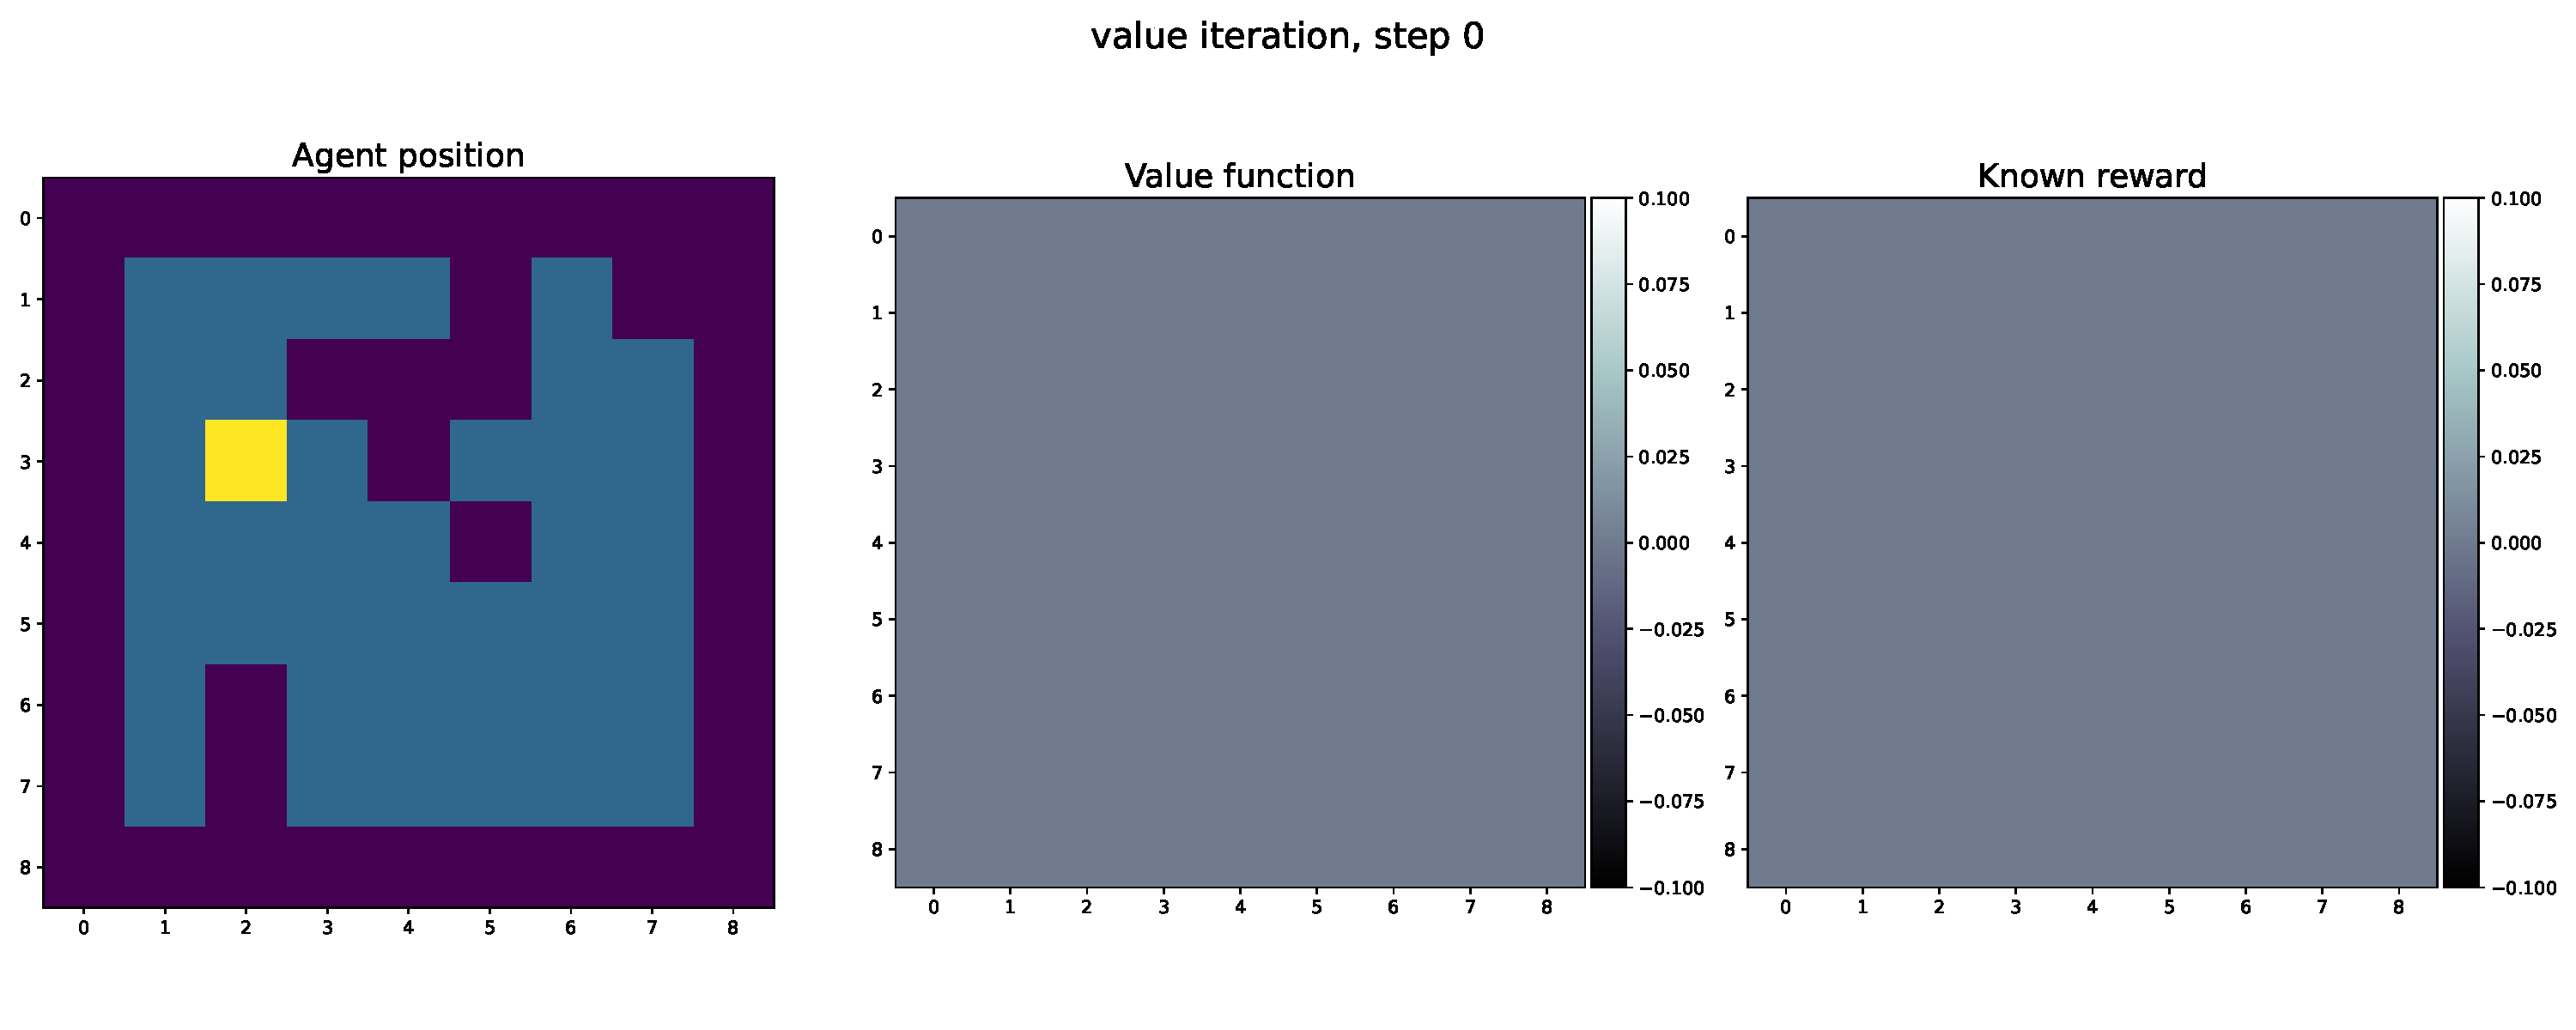
\includegraphics[width=1.05\textwidth]{value_iteration_step_0}
	\caption{Iteration 0}
	\label{fig:}
\end{figure}
\end{frame}


\begin{frame}{Value iteration}
    At step $3$ a reward is found, information propagates.
\begin{figure}[htpb]
	\centering
	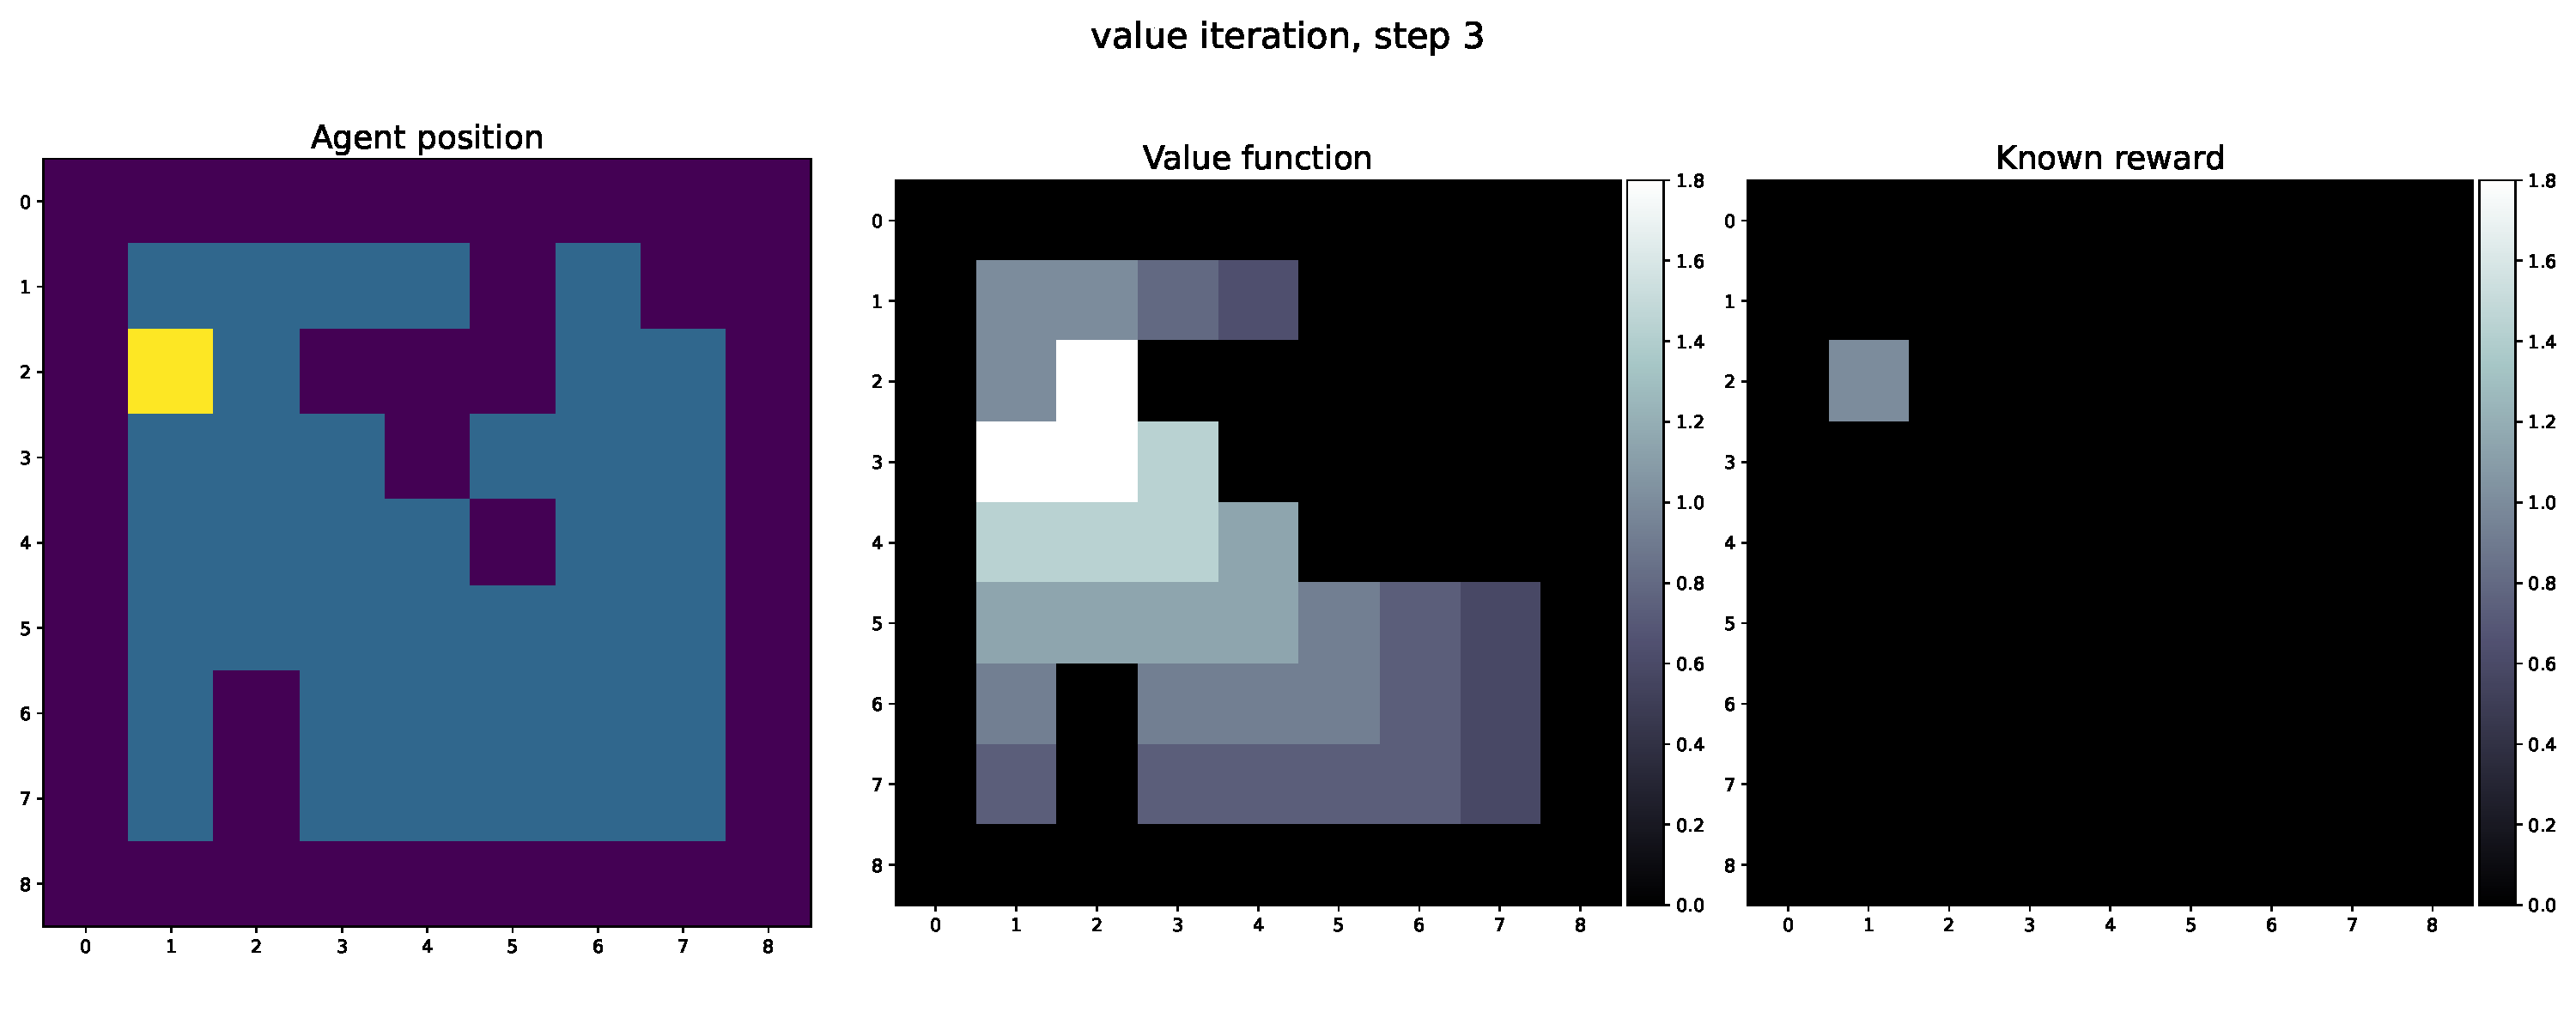
\includegraphics[width=1.05\textwidth]{value_iteration_step_3}
	\caption{Iteration 3}
	\label{fig:}
\end{figure}
\end{frame}


\begin{frame}{Value iteration}
    Information propagation.
\begin{figure}[htpb]
	\centering
	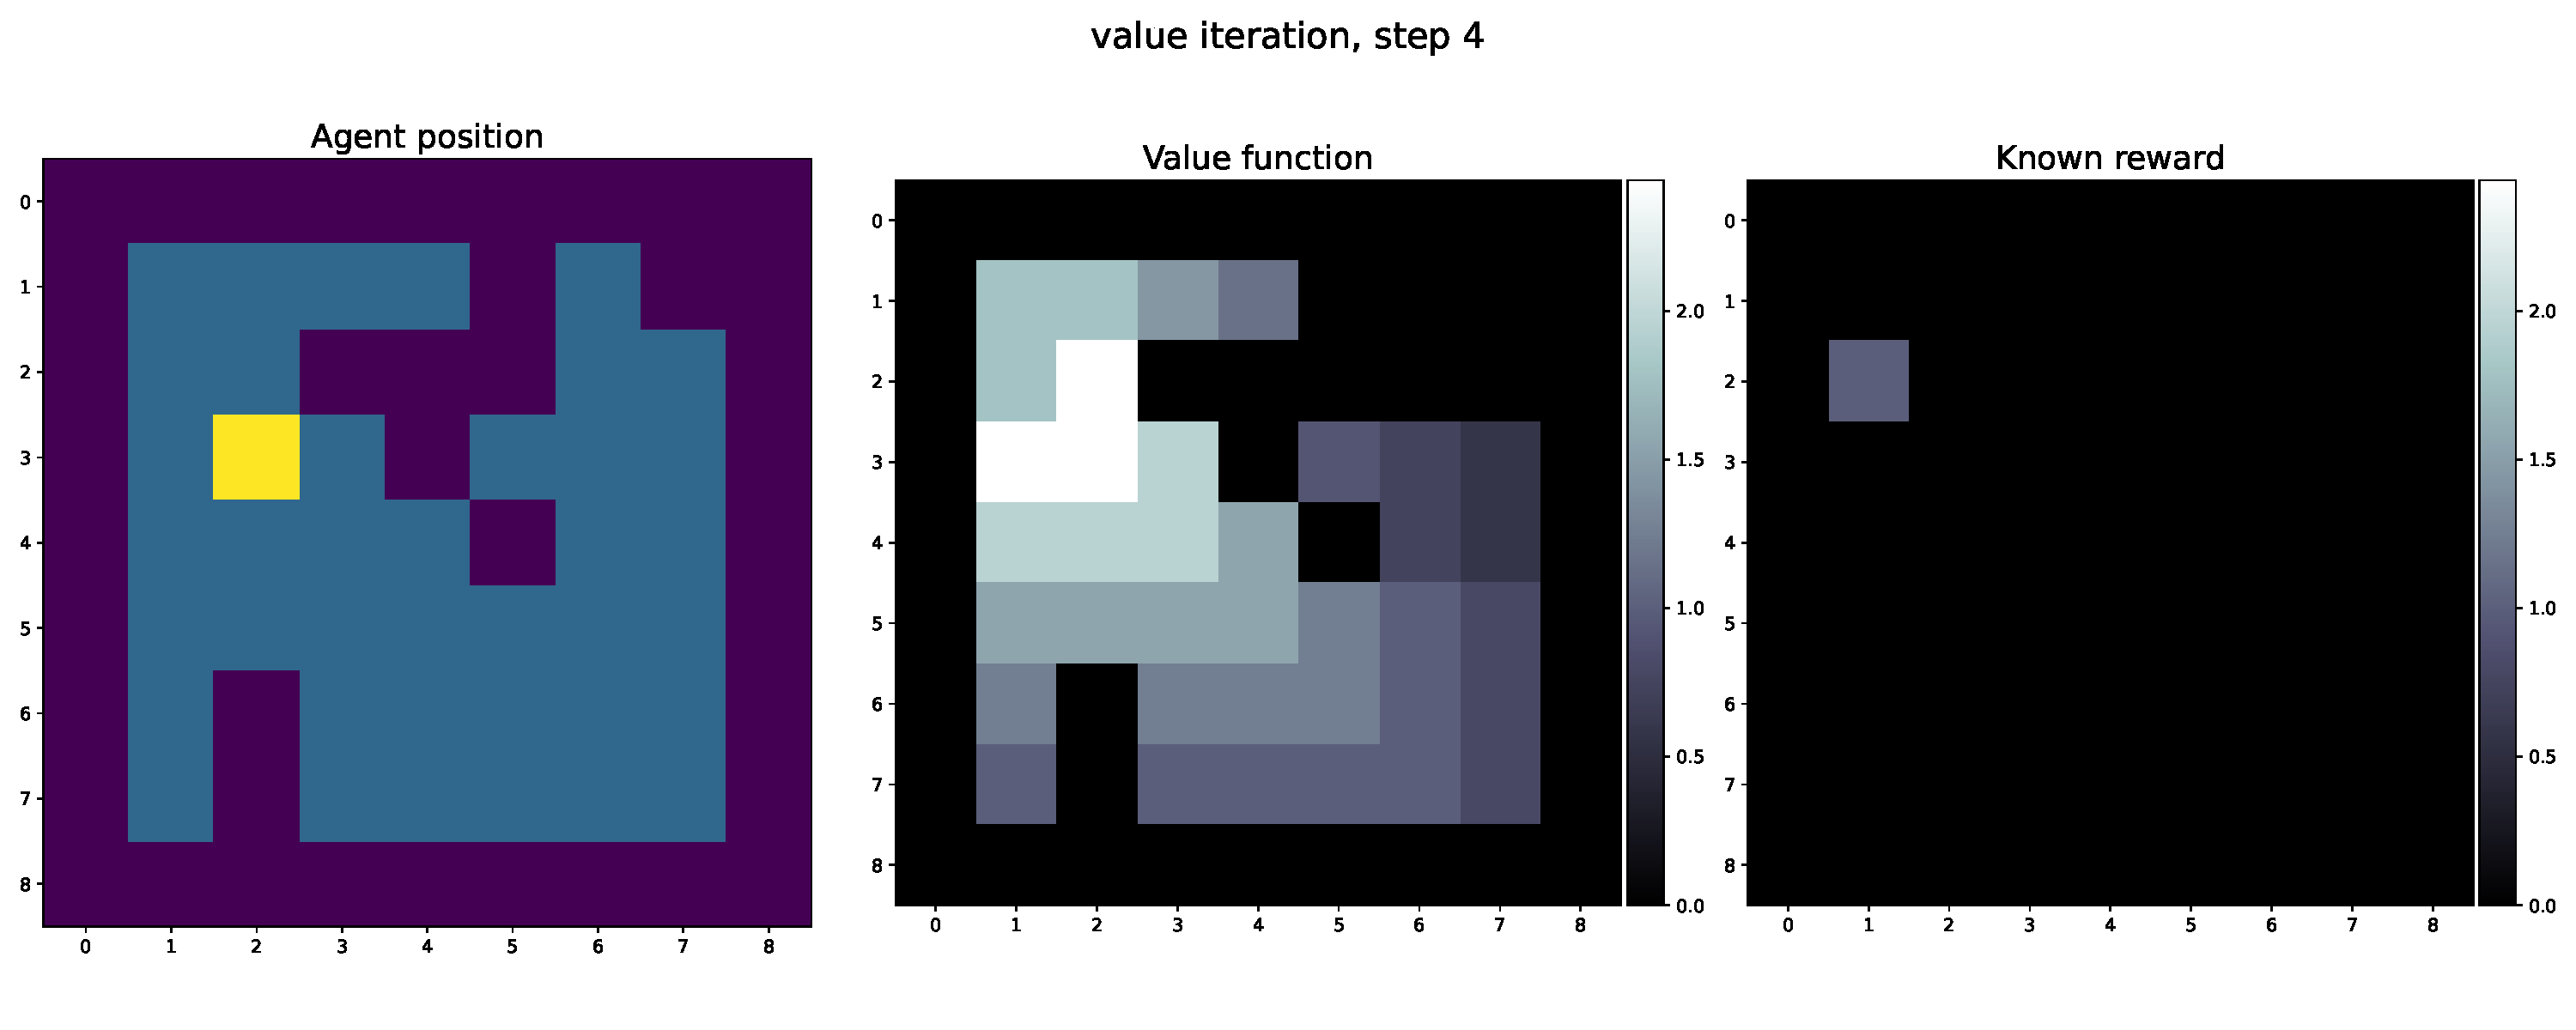
\includegraphics[width=1.05\textwidth]{value_iteration_step_4}
	\caption{Iteration 4}
	\label{fig:}
\end{figure}
\end{frame}


\begin{frame}{Value iteration}
\begin{figure}[htpb]
	\centering
	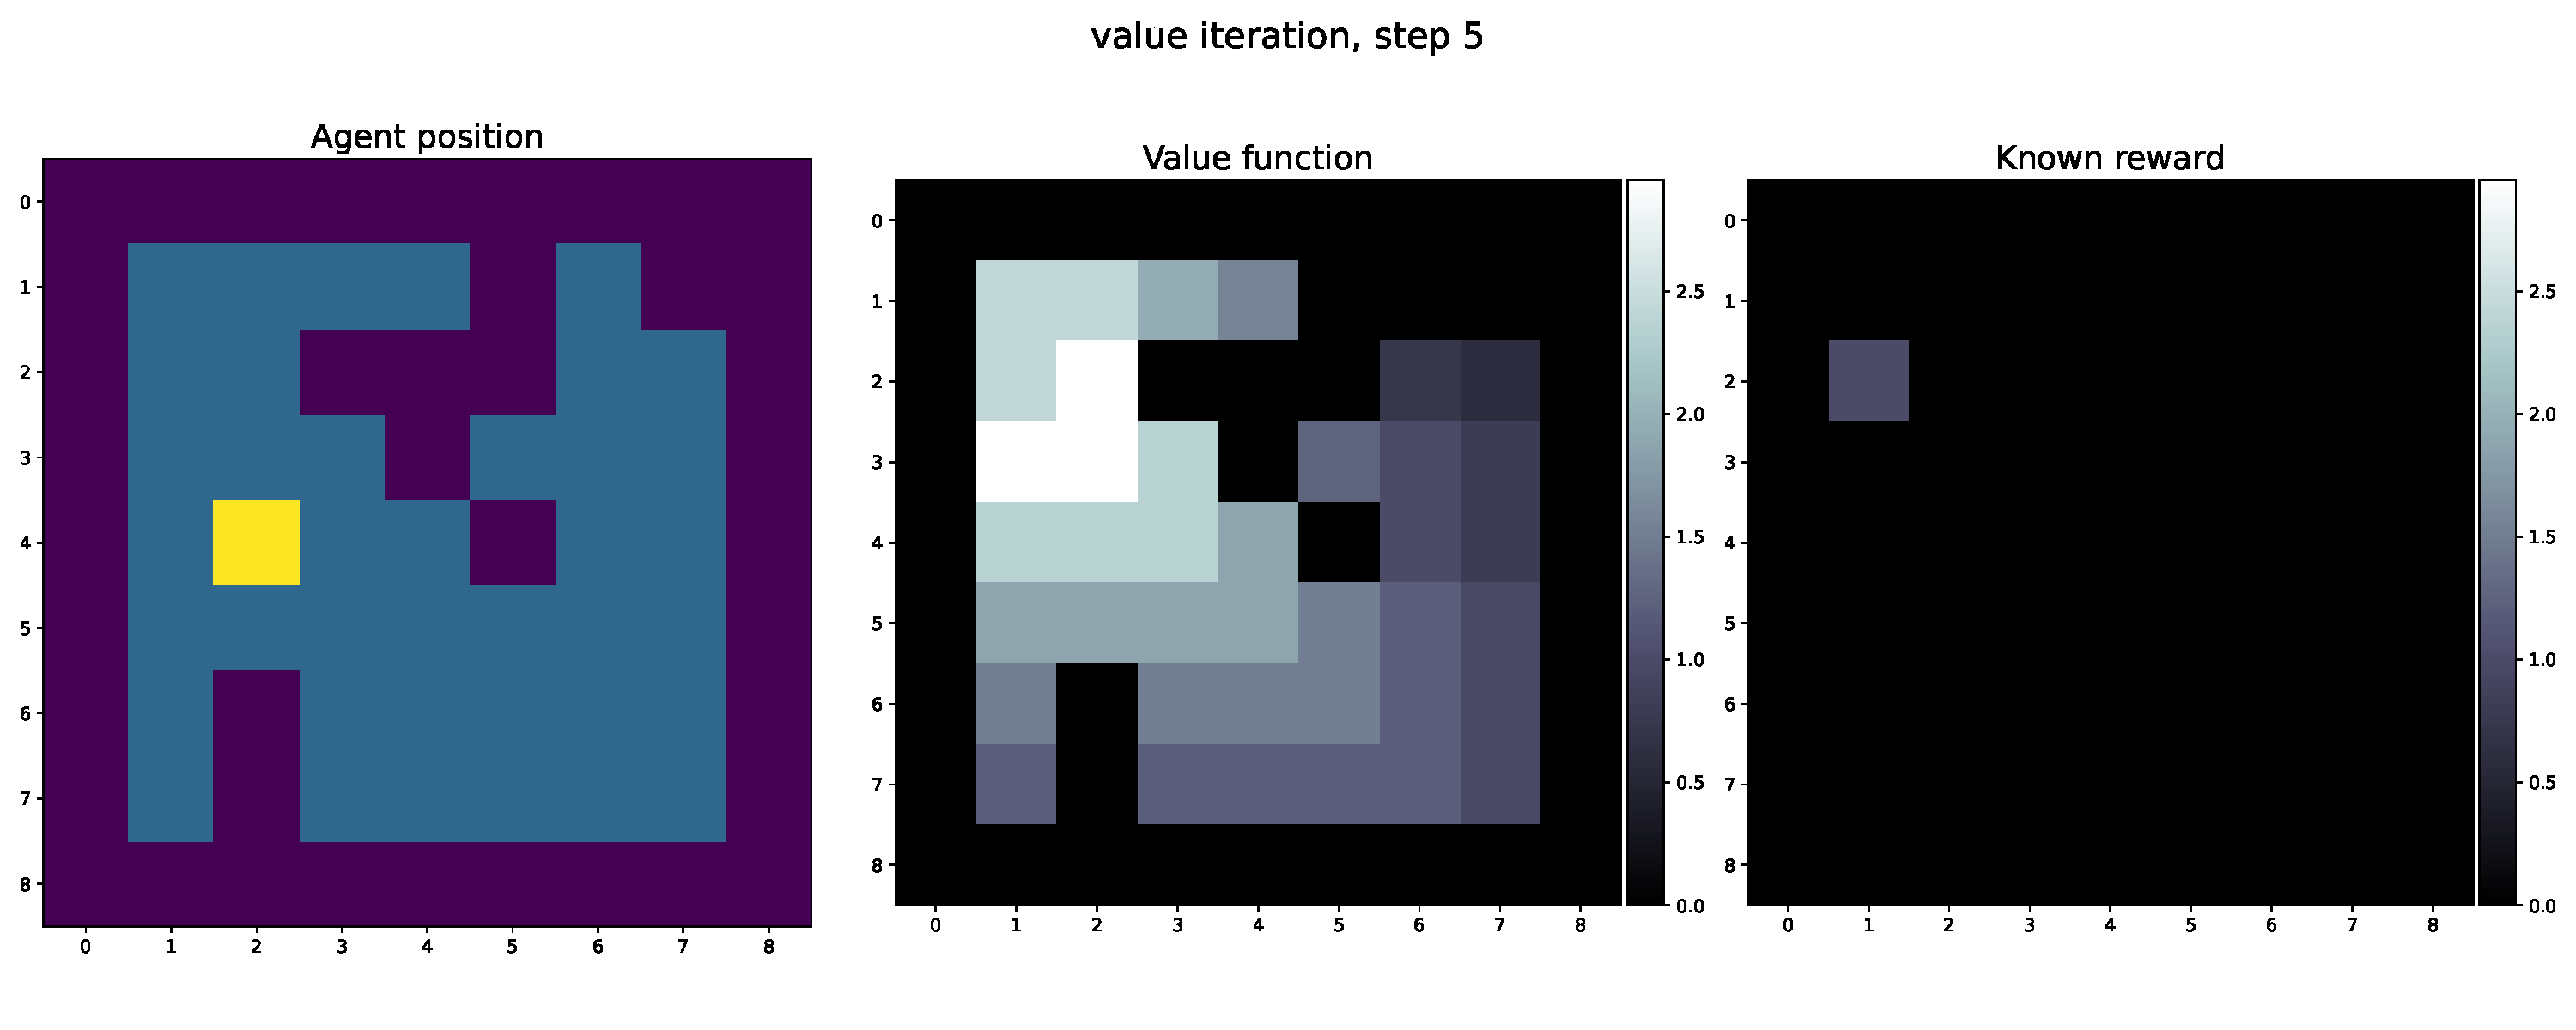
\includegraphics[width=1.05\textwidth]{value_iteration_step_5}
	\caption{Iteration 5}
	\label{fig:}
\end{figure}
\end{frame}


\begin{frame}{Value iteration}
    Another reward is found at step 7.
\begin{figure}[htpb]
	\centering
	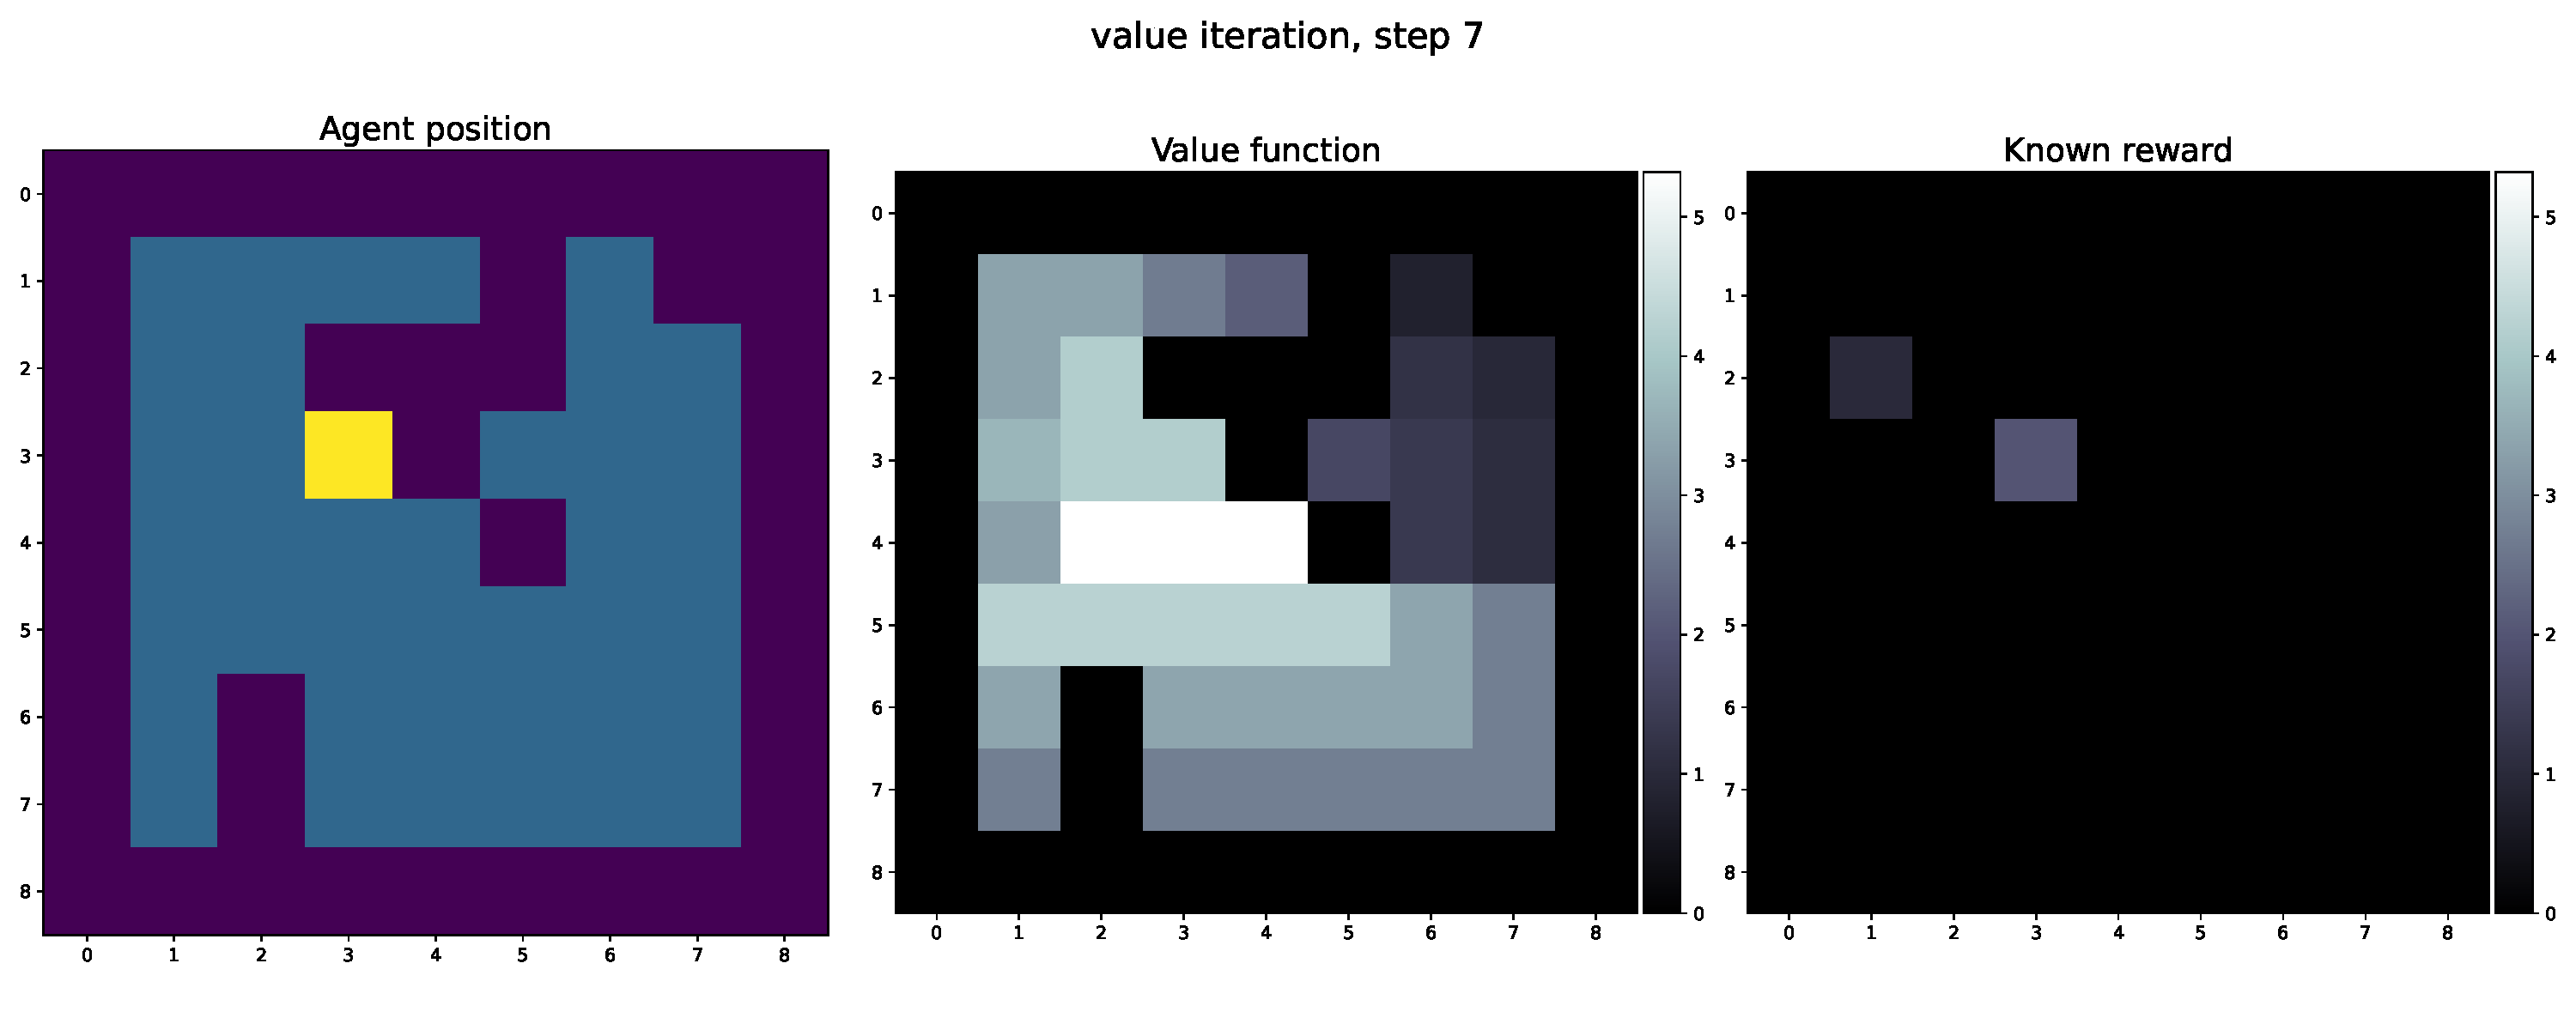
\includegraphics[width=1.05\textwidth]{value_iteration_step_7}
	\caption{Iteration 7}
	\label{fig:}
\end{figure}
\end{frame}


\begin{frame}{Value iteration}
\begin{figure}[htpb]
	\centering
	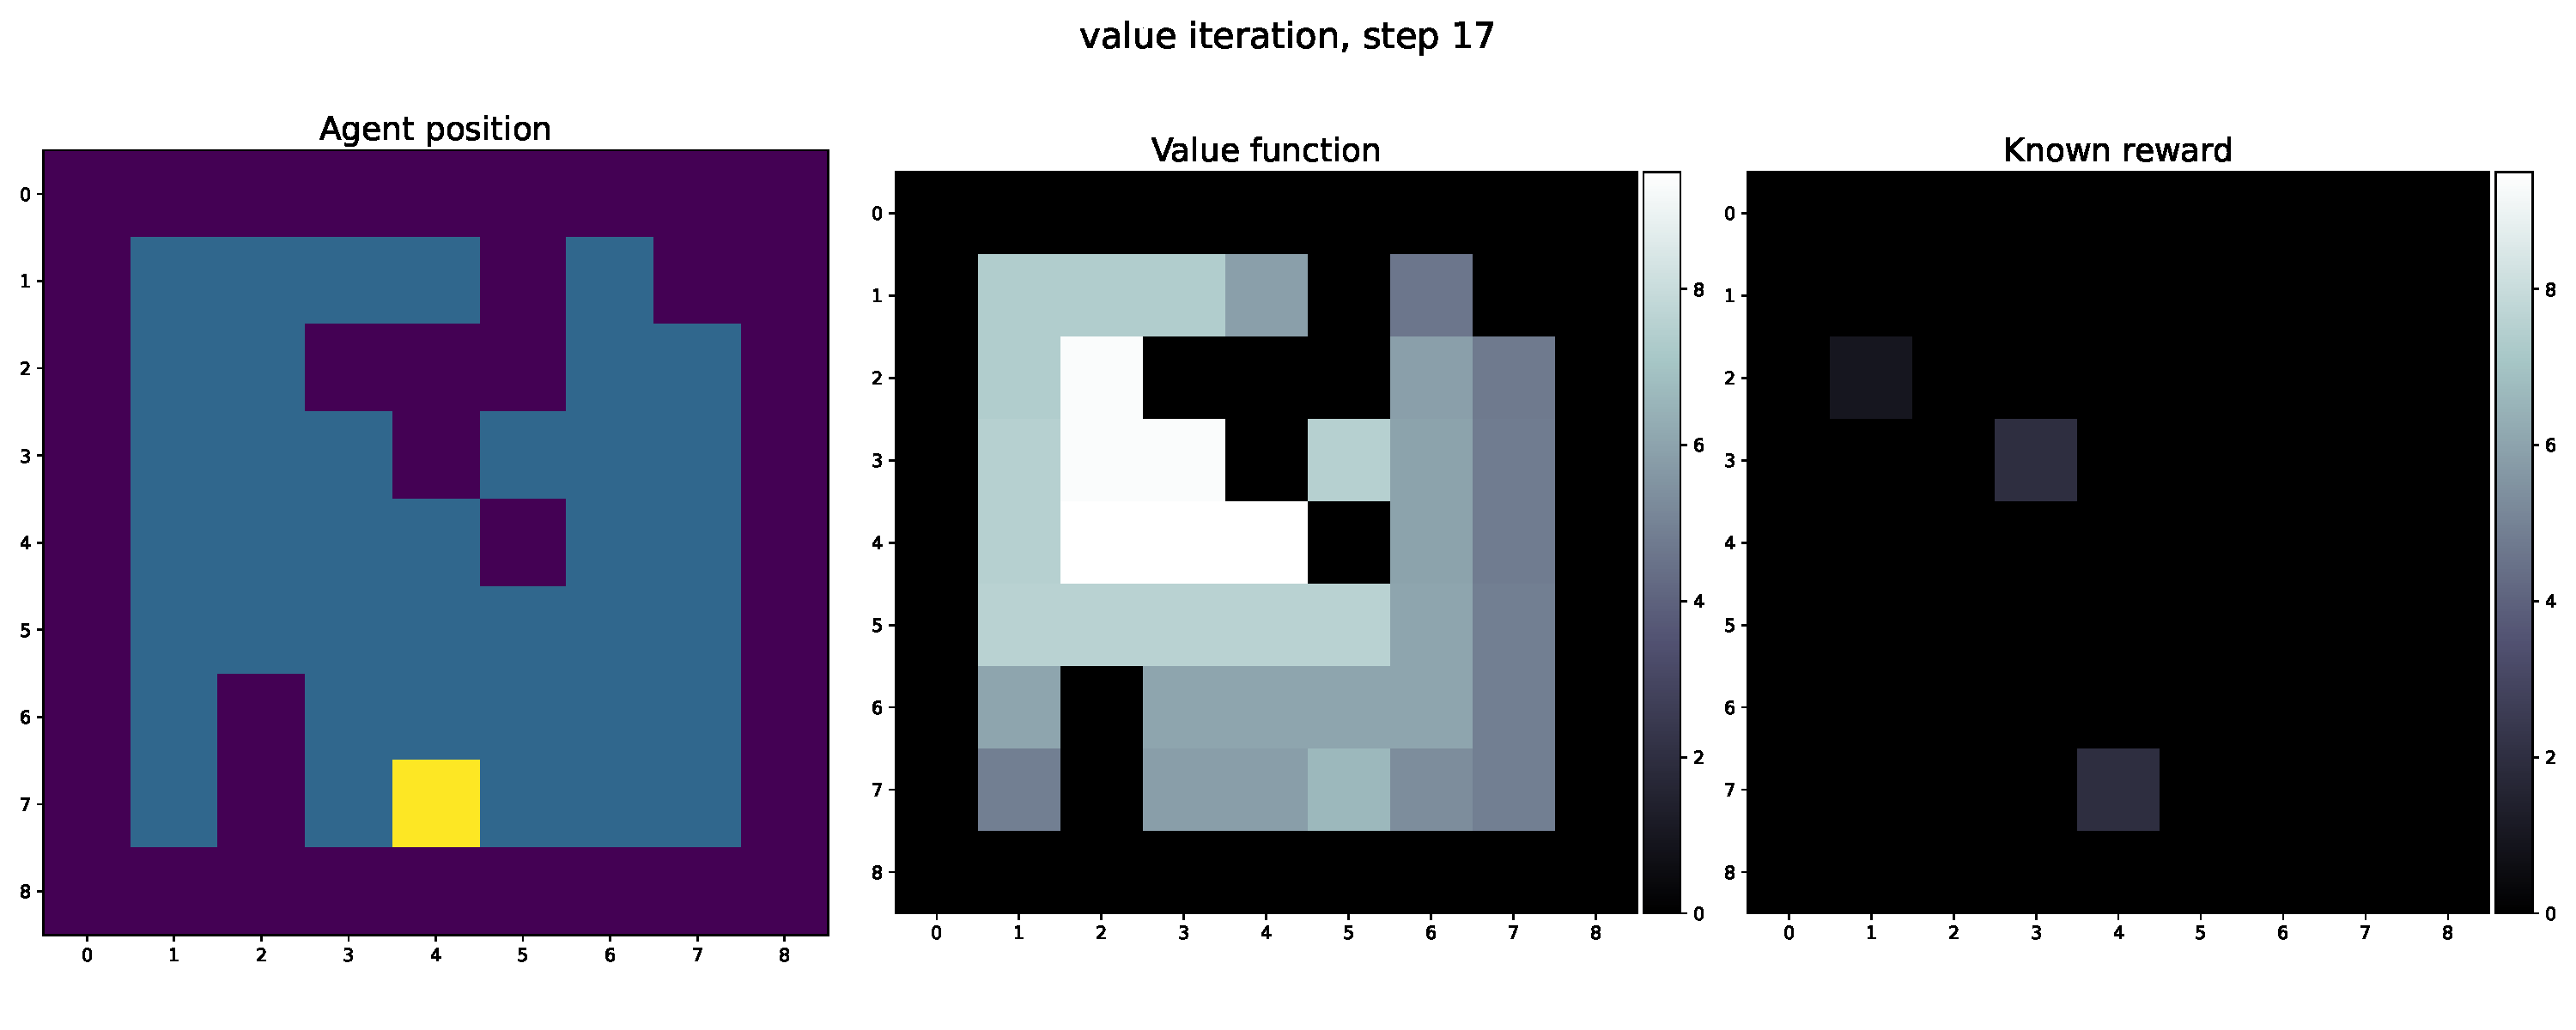
\includegraphics[width=1.05\textwidth]{value_iteration_step_17}
	\caption{Iteration 17}
	\label{fig:}
\end{figure}
\end{frame}


\begin{frame}{Value iteration}
\begin{figure}[htpb]
	\centering
	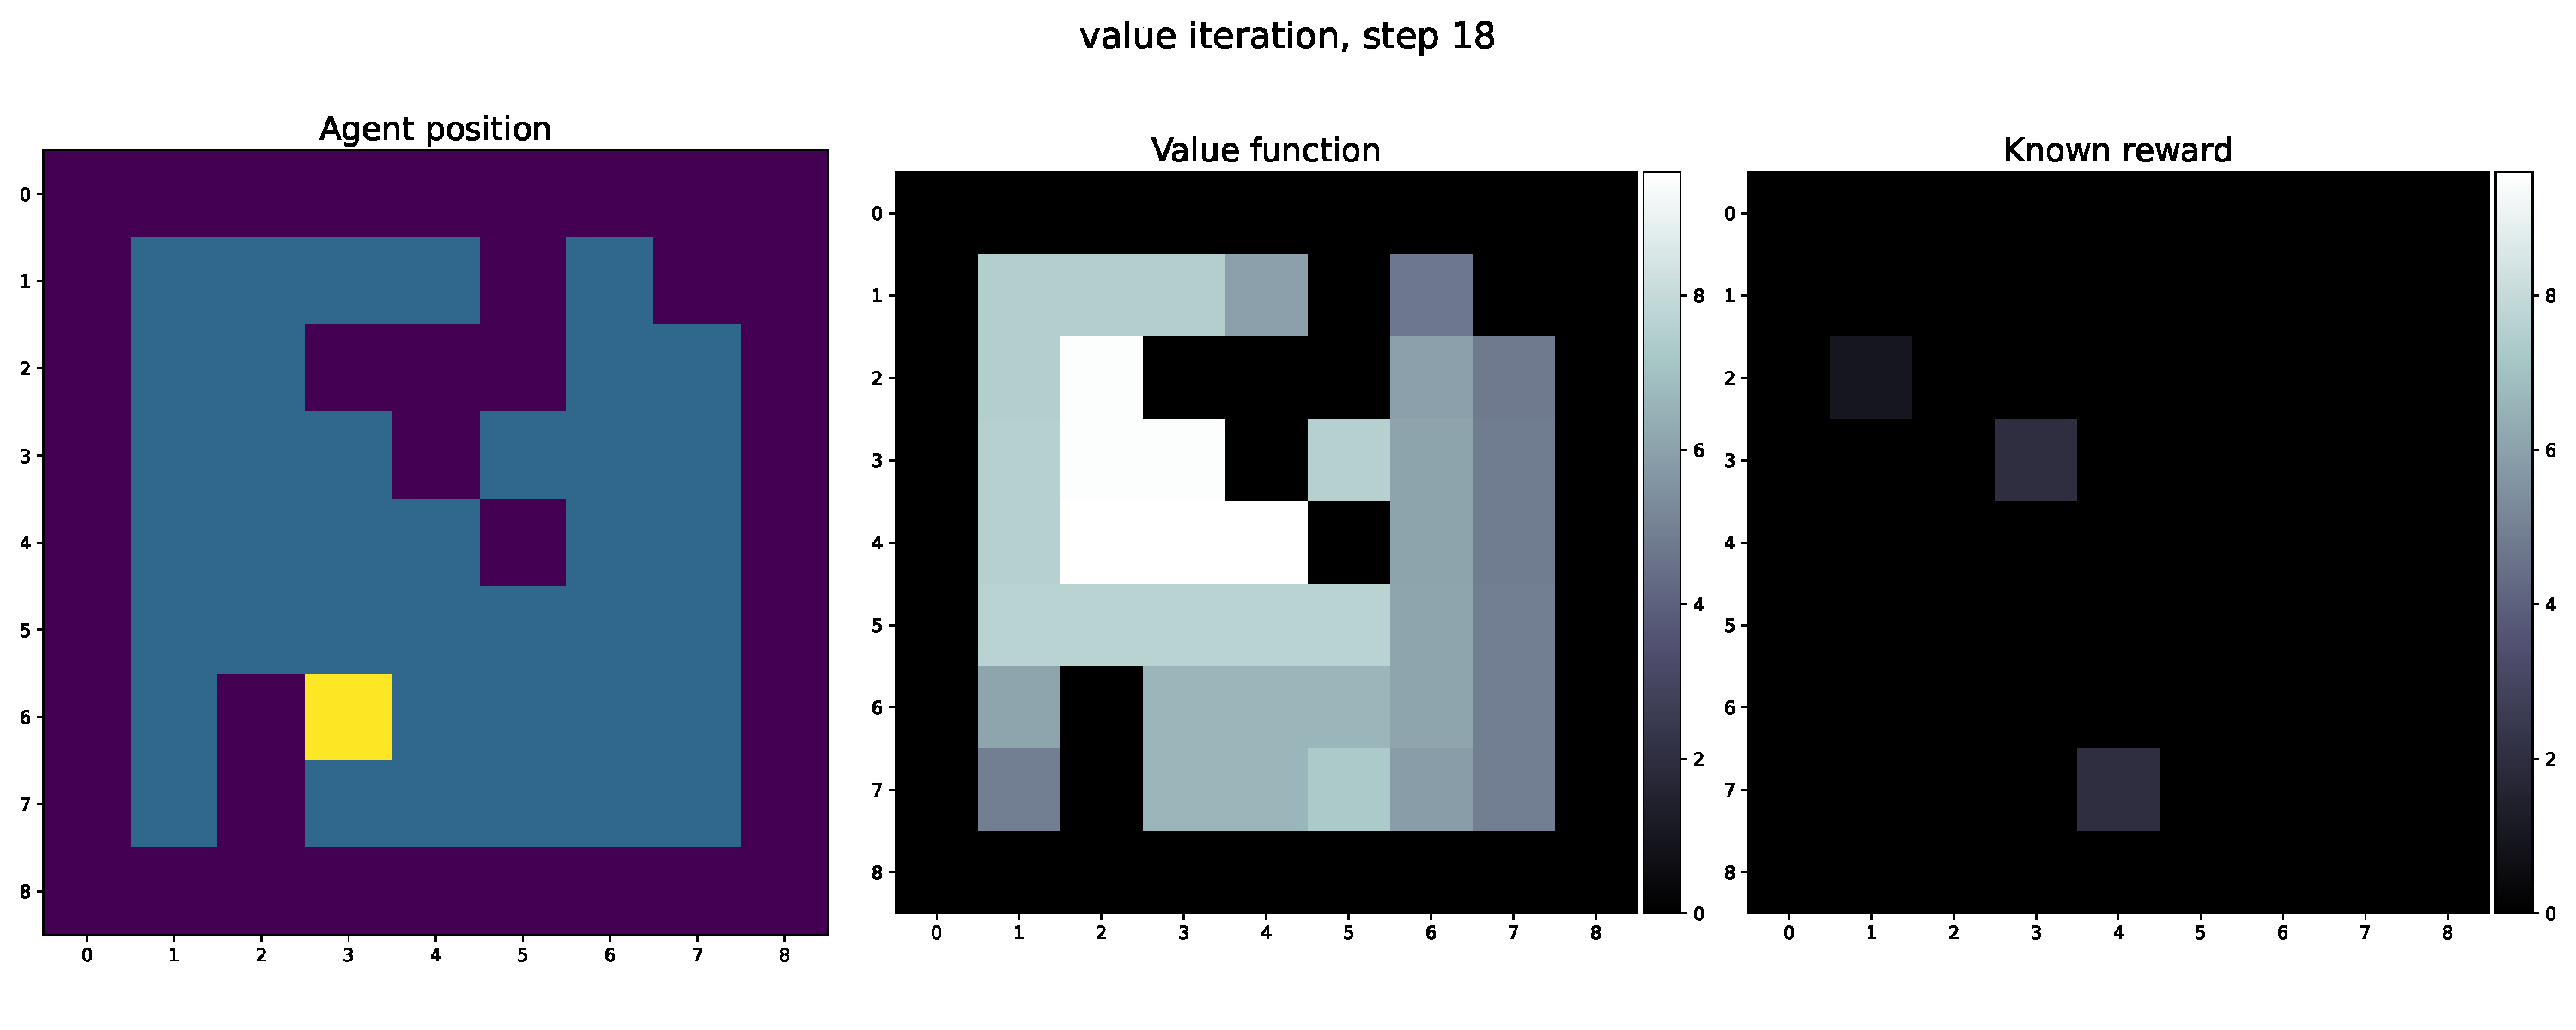
\includegraphics[width=1.05\textwidth]{value_iteration_step_18}
	\caption{Iteration 18}
	\label{fig:}
\end{figure}
\end{frame}


\begin{frame}{Value iteration}
\begin{figure}[htpb]
	\centering
	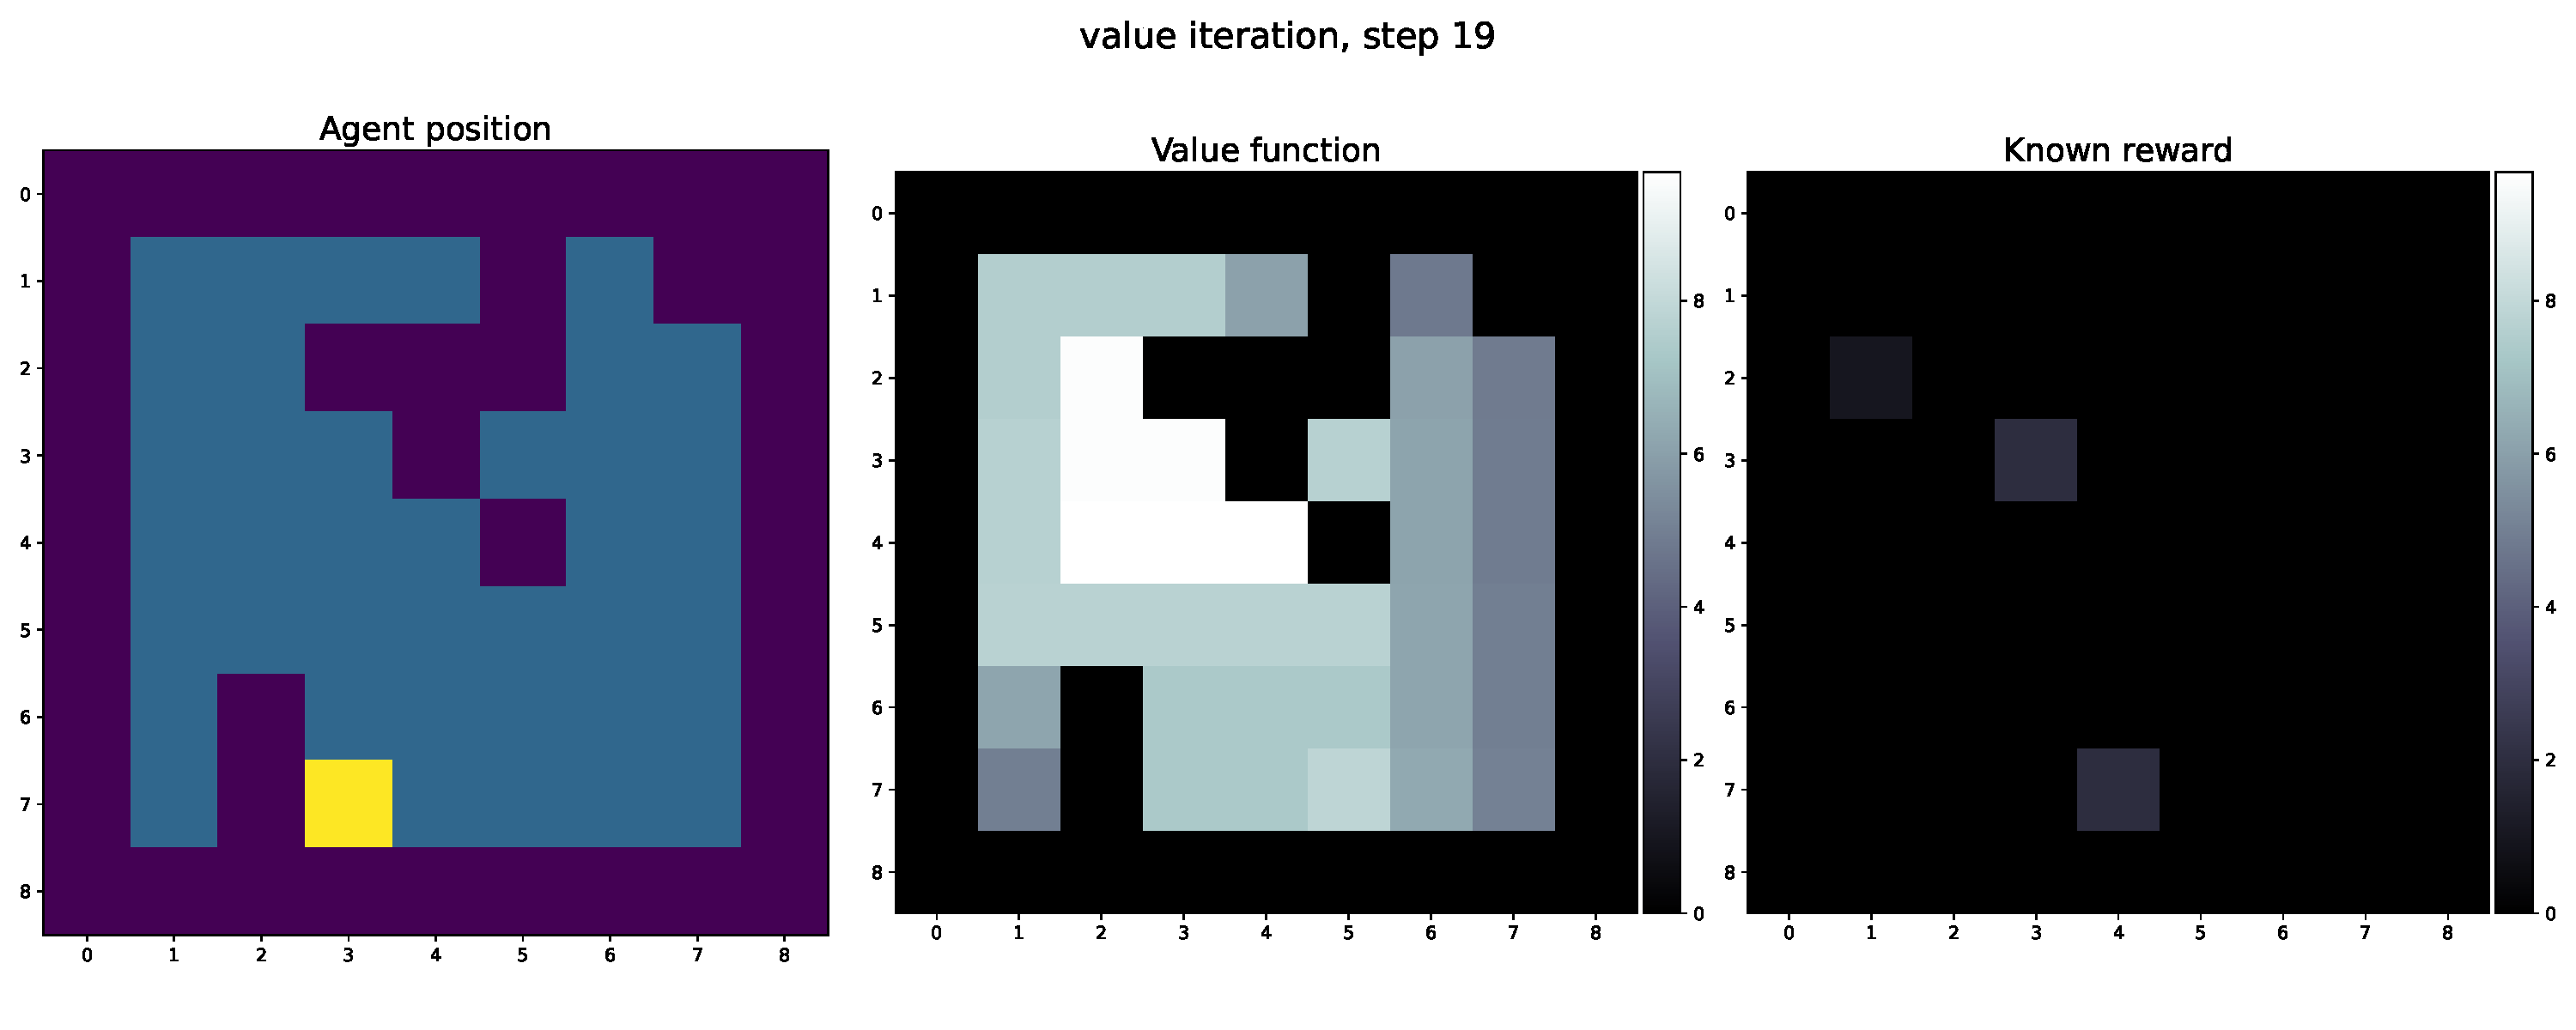
\includegraphics[width=1.05\textwidth]{value_iteration_step_19}
	\caption{Iteration 19}
	\label{fig:}
\end{figure}
\end{frame}


\begin{frame}{Value iteration}
         After a number of iterations, we observe the convergence of the value function.
\begin{figure}[htpb]
	\centering
	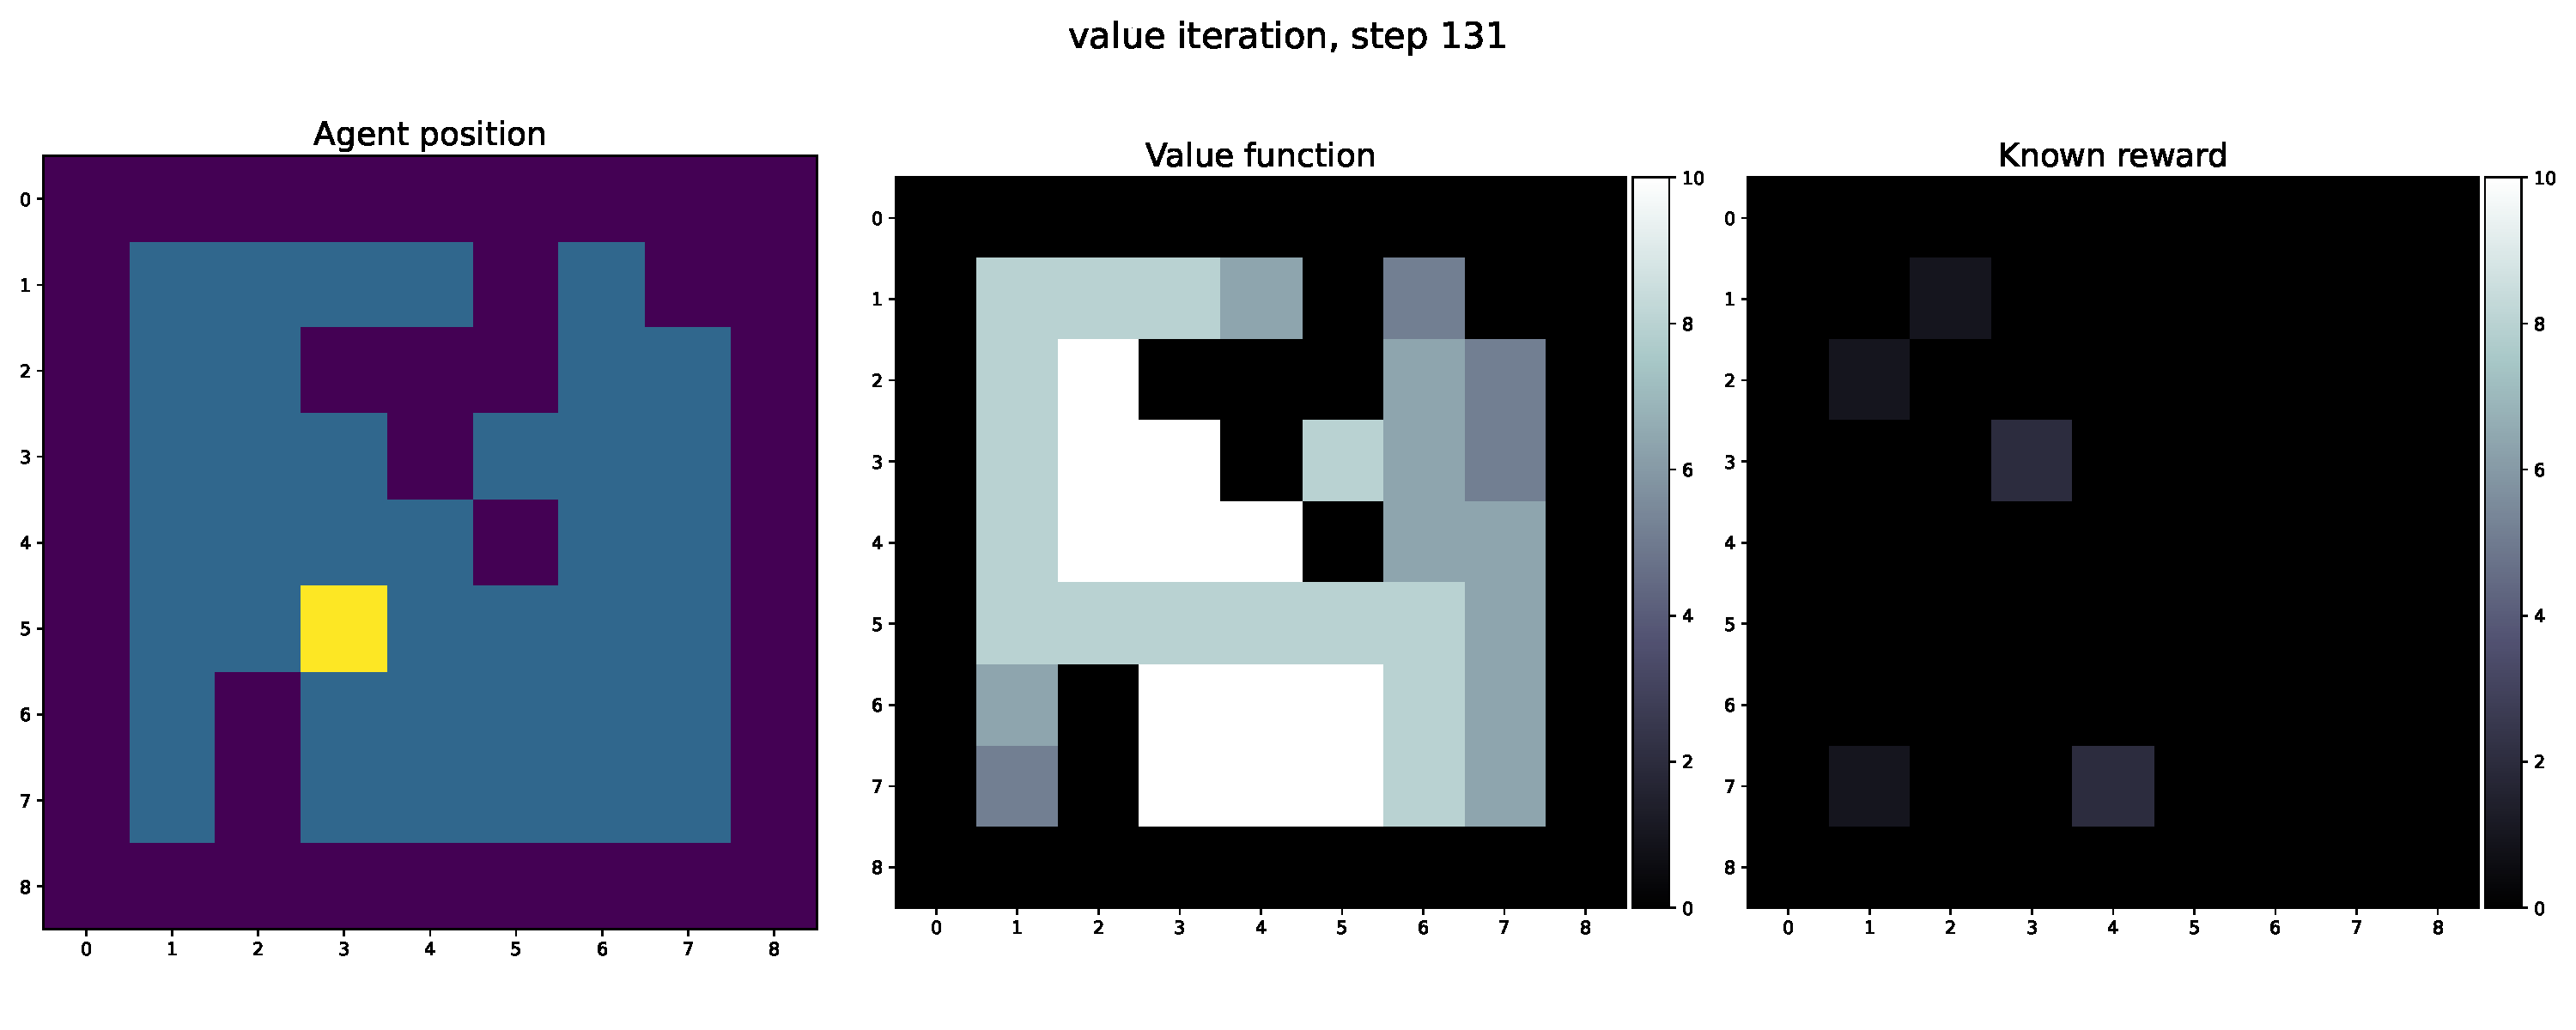
\includegraphics[width=1.05\textwidth]{value_iteration_step_131}
	\caption{Iteration 131}
	\label{fig:}
\end{figure}
\end{frame}

\begin{frame}
    \exercice{}
   \begin{itemize}
	\item \textbf{{cd 2\textunderscore reinforcement\textunderscore learning/}} 
	\item We store the data about the world in \textbf{{.npy}} files (optionally, you can generate a different world !)
       \item In \textbf{{value\textunderscore iteration.py}}, modify:
	   \begin{itemize}
	   	\item \textbf{{move\textunderscore agent()}} so that the agent is
           randomly moved at each time step.
	    \item \textbf{{update\textunderscore value\textunderscore
            function()}} in order to update the value function according to the
            Bellman equation, and run the algorithm until convergence of the
            value function.
	   \end{itemize}
   \end{itemize}
\end{frame}

\begin{frame}{Optimal policy}
   \begin{figure}[htpb]
       \centering
       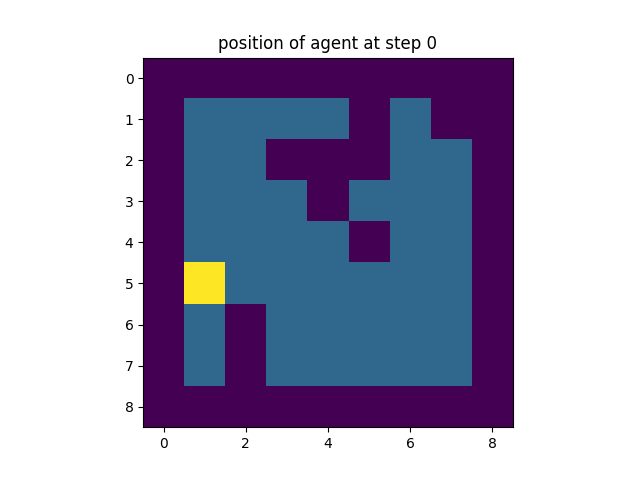
\includegraphics[width=0.7\linewidth]{agent_position_travel_3_step_0}
       \caption{After learning hte optimal policy, the agent can go to the reward.}
       \label{fig:}
   \end{figure} 
\end{frame}
\begin{frame}{Optimal policy}
   \begin{figure}[htpb]
       \centering
       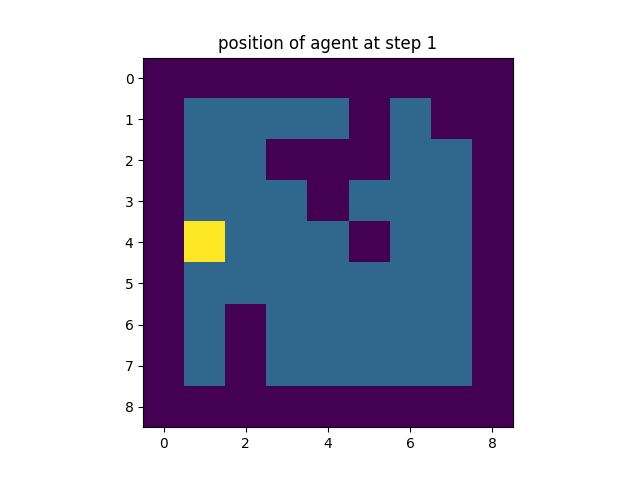
\includegraphics[width=0.7\linewidth]{agent_position_travel_3_step_1}
       \caption{After learning, the agent can go to the reward.}
       \label{fig:}
   \end{figure} 
\end{frame}
\begin{frame}{Optimal policy}
   \begin{figure}[htpb]
       \centering
       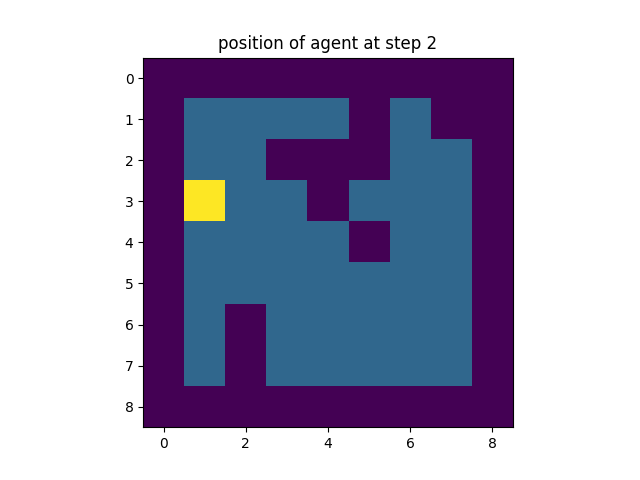
\includegraphics[width=0.7\linewidth]{agent_position_travel_3_step_2}
       \caption{After learning, the agent can go to the reward.}
       \label{fig:}
   \end{figure} 
\end{frame}
\begin{frame}{Optimal policy}
   \begin{figure}[htpb]
       \centering
       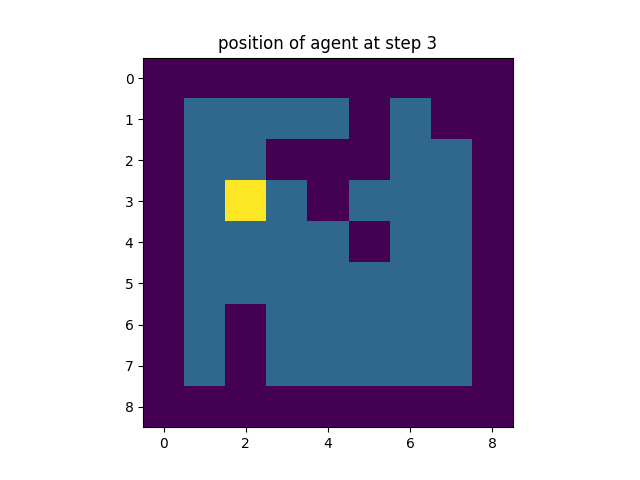
\includegraphics[width=0.7\linewidth]{agent_position_travel_3_step_3}
       \caption{After learning, the agent can go to the reward.}
       \label{fig:}
   \end{figure} 
\end{frame}
\begin{frame}{Optimal policy}
   \begin{figure}[htpb]
       \centering
       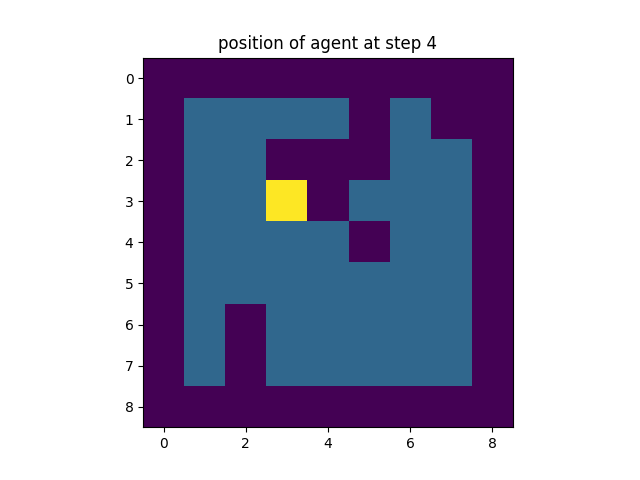
\includegraphics[width=0.7\linewidth]{agent_position_travel_3_step_4}
       \caption{After learning, the agent can go to the reward.}
       \label{fig:}
   \end{figure} 
\end{frame}

\begin{frame}{Optimal policy}
   \begin{figure}[htpb]
       \centering
       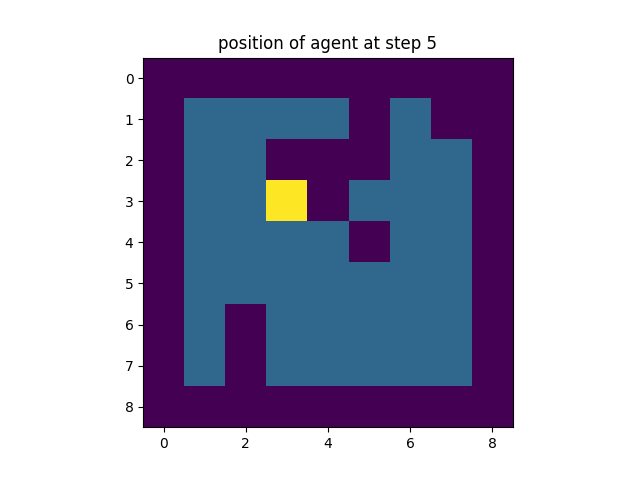
\includegraphics[width=0.7\linewidth]{agent_position_travel_3_step_5}
       \caption{After learning, the agent can go to the reward.}
       \label{fig:}
   \end{figure} 
\end{frame}

\section{Policy iteration}


%\begin{frame}{Policy Iteration}
%    \begin{itemize}
%    \item \textbf{{Policy iteration}} is another method that is slightly
%        different. 
%    \item It consists in two steps : 
%        \begin{itemize}
%            \item \textbf{{Policy evaluation}} 
%        \end{itemize}
%    \end{itemize}
%\end{frame}
%
%\begin{frame}{Policy Iteration}
%    \begin{itemize}
%    \item \textbf{{Policy iteration}} is another method that is slightly
%        different. 
%    \item It consists in two steps : 
%        \begin{itemize}
%            \item \textbf{{Policy evaluation}} 
%            \item \textbf{{Policy improvement}} 
%        \end{itemize}
%    \end{itemize}
%\end{frame}
%
%
%\begin{frame}
%    \exercice{}
%    \begin{itemize}
%        \item Pease use the file \textbf{{policy\textunderscore iteration.py}}  in order to perform the algorithm.
%	    \item Add randomness to the actions of the agent to \textbf{{guarantee exploration}}.
%    \end{itemize}
%\end{frame}

\section{Discussion}

\begin{frame}{Multiple paradigms}
   \begin{itemize}
       \item Reinforcement learning has many variants.
        \item In the ones we studied, a model of the consequence of our actions was
            known.
        \item This is not always the case.
   \end{itemize} 
\end{frame}

\subsection{Temporal Difference learning}%
\label{sub:temporal_difference_learning}

\begin{frame}{Temporal difference learning}
\begin{itemize}
    \item In temporal difference learning, the agent does not know a
        \textbf{{model}} of its world.
    \item But it can still learn the value function with the \textbf{{TD (temporal difference) updates}} 
    \begin{equation} V(S_t)\leftarrow
V(S_t)+\alpha[R_{t+1}+\gamma V(S_{t+1})-V(S_t)] \label{eq:td0}
    \end{equation}
\end{itemize}
\end{frame}


\subsection{Additional considerations}%
\label{sec:kk}

\begin{frame}{Monte Carlo methods}
    Monte Carlo methods can be used in Reinforcement Learning to estimate
        some expected values (such as the expected reward in a given state).
\end{frame}

% \begin{frame}{Q learnin}
%     
% \end{frame}

%\begin{frame}{Local vs global updates}
%    
%\end{frame}

\begin{frame}{Actor critic methods}
\begin{itemize}
    \item Sometimes you can use \textbf{{two}} policies
        \begin{itemize}
            \item the \textbf{{behavior policy}} provides actions and guarantees
                exploration
            \item the \textbf{{target policy}} is the optimal policy learned in
                parallel by the agent, that would be used in exploitation mode.
        \end{itemize}
\end{itemize}    
\end{frame}

\begin{frame}{Tabular case and continous case}
   \begin{itemize}
       \item We studied \textbf{{finite}} (and thus discrete situations).
        \item However, RL can also be applied to continuous state / discrete
            action spaces (DQN) 
        \item And even to continous state / continous action spaces (DDPG)
            \cite{Bengio2009} .
   \end{itemize} 
\end{frame}




\begin{frame}[allowframebreaks]
\frametitle{References}
\bibliographystyle{apalike}
\bibliography{epitech.bib} 
\end{frame}

\end{document} 
